\documentclass[11pt,a4paper]{article}

\usepackage[margin=1in]{geometry}
\usepackage{microtype}
\usepackage{graphicx}
\usepackage[table]{xcolor}
% ---- revision highlighting ----
% IMPORTANT: highlighted mode requires the LuaLaTeX compiler.
\usepackage{iftex}
\ifLuaTeX
  \usepackage{luacolor}
  \usepackage{lua-ul}
\fi
\colorlet{RevisionHighlight}{yellow!55}

% ============================================================
%  CHANGE-MARKING SWITCH
%  Highlighted version : \highlighttrue   (yellow background)
%  Clean version       : \highlightfalse  (no marks)
% ============================================================
\newif\ifhighlight
\highlighttrue
%\highlightfalse

% Only changes made for the present review round use \add{...},
% \addeq{...}, or \revtableon/\revtableoff. Earlier revisions
% are hard-coded as ordinary manuscript text.
\NewDocumentCommand{\add}{+m}{%
  \ifhighlight
    \ifLuaTeX
      \highLight[RevisionHighlight]{#1}%
    \else
      \PackageError{Revision highlighting}{Highlighted mode requires LuaLaTeX}{Set the Overleaf compiler to LuaLaTeX, or use \string\highlightfalse\space for the clean version.}%
      #1%
    \fi
  \else
    #1%
  \fi
}

% Display equations cannot safely be placed inside a line-highlighting command,
% so new display equations use a yellow background box in highlighted mode.
\NewDocumentCommand{\addeq}{+m}{%
  \ifhighlight
    \[
      \colorbox{RevisionHighlight}{\(\displaystyle #1\)}
    \]
  \else
    \[
      #1
    \]
  \fi
}

% New tables are marked by yellow cell backgrounds in highlighted mode.
\newcommand{\revtableon}{%
  \begingroup
  \ifhighlight\rowcolors{1}{RevisionHighlight}{RevisionHighlight}\fi
}
\newcommand{\revtableoff}{%
  \endgroup
}

\newcommand{\del}[1]{}       % deleted text is always removed
\newcommand{\delnote}[1]{}   % editorial notes are always removed


\usepackage{booktabs}
\usepackage{tabularx}
\usepackage{array}
\usepackage{adjustbox}
\usepackage{amsmath,amssymb}
\usepackage{siunitx}
\usepackage[version=4]{mhchem}
\usepackage[colorlinks=true,linkcolor=blue!50!black,citecolor=blue!50!black,urlcolor=blue!50!black]{hyperref}
\usepackage[nameinlink,noabbrev]{cleveref}
\usepackage{caption}
\usepackage{tocloft}
\usepackage{placeins}
\usepackage{float}

\usepackage[numbers,sort&compress]{natbib}

\hypersetup{
colorlinks=true,
linkcolor=blue!50!black,
citecolor=blue!50!black,
urlcolor=blue!50!black
}

\captionsetup{font=small,labelfont=bf}
\renewcommand{\thefigure}{S\arabic{figure}}
\renewcommand{\thetable}{S\arabic{table}}
\renewcommand{\theequation}{S\arabic{equation}}
\setlength{\cftbeforesecskip}{4pt}

\newcommand{\Htwo}{\ce{H2}}
\newcommand{\COtwo}{\ce{CO2}}
\newcommand{\CHfour}{\ce{CH4}}
\newcommand{\Ntwo}{\ce{N2}}
\newcommand{\TSA}{temperature-swing adsorption}
\newcommand{\PSA}{pressure-swing adsorption}

\sisetup{detect-all=true,per-mode=symbol,range-phrase=--,range-units=single}

% Switch: edit \highlighttrue / \highlightfalse in preamble.
\begin{document}

\begin{titlepage}
\centering
\vspace*{1.5cm}

{\Large\bfseries Supporting Information\par}

\vspace{0.8cm}

{\large\bfseries Biomass gasification determines MOF--zeolite ranking in hydrogen-stream purification screening\par}

\vspace{0.8cm}

{\normalsize
Zahra Soltani,$^{1,\dagger}$
Shayan Abaei,$^{2,\dagger}$
Mohammadsaleh Hoseinzadeh,$^{3,\dagger}$
Fahimeh Hooriabad Saboor,$^{1,*}$
Hosein Alimardani,$^{4}$
Seyed Parsa Amouzesh,$^{5}$
and Mehrdad Asgari$^{6,*}$\par}

\vspace{0.8cm}

\begin{minipage}{0.94\textwidth}
\small
\centering
$^{1}$Department of Chemical Engineering, University of Mohaghegh Ardabili, Ardabil, Iran\\
$^{2}$School of Chemical Engineering, College of Engineering, University of Tehran, Tehran, Iran\\
$^{3}$Department of Chemical Engineering, Faculty of Engineering, Ferdowsi University of Mashhad, Mashhad 9177948944, Iran\\
$^{4}$Faculty of Engineering, University of Tehran, Tehran, Iran\\
$^{5}$Department of Chemical and Biological Engineering, Illinois Institute of Technology, Chicago, IL 60616, USA\\
$^{6}$Lucy Cavendish College, University of Cambridge, Cambridge CB3 0BU, United Kingdom\\[0.8em]

$^{\dagger}$These authors contributed equally to this work.\\[0.4em]
$^{*}$Corresponding authors: Fahimeh Hooriabad Saboor,
\href{mailto:f.saboor@uma.ac.ir}{f.saboor@uma.ac.ir};
Mehrdad Asgari,
\href{mailto:ma2000@cam.ac.uk}{ma2000@cam.ac.uk}
\end{minipage}

\vfill

{\small This Supporting Information contains the detailed process flowsheet,
reaction assumptions, stream tables, upstream sensitivity maps, adsorption
equations, fitted Langmuir parameters for HKUST-1 and Cu-TDPAT, the
Ruthven--Sips parameter set for Zeolite~13X, isotherm and working-capacity
panels, tree-ensemble surrogate held-out performance and TreeSHAP attribution,
main-text figure-panel guide, process-conditioned material-selection matrix,
a pressure-swing robustness check, and a $\eta$/$t_{\mathrm{cycle}}$
robustness analysis. These materials support a comparative equilibrium-screening
interpretation rather than a final cyclic column-design claim.}

\end{titlepage}

\tableofcontents
\newpage

\section{Process flowsheet and base-case stream data}

\subsection{Detailed Aspen HYSYS flowsheet}

The detailed Aspen HYSYS flowsheet documents the unit-level gasification,
recycle and separation structure used to generate the \TSA{} feed composition.
The simplified schematic is Fig.~1 of the main manuscript.

\begin{figure}[htbp]
\centering
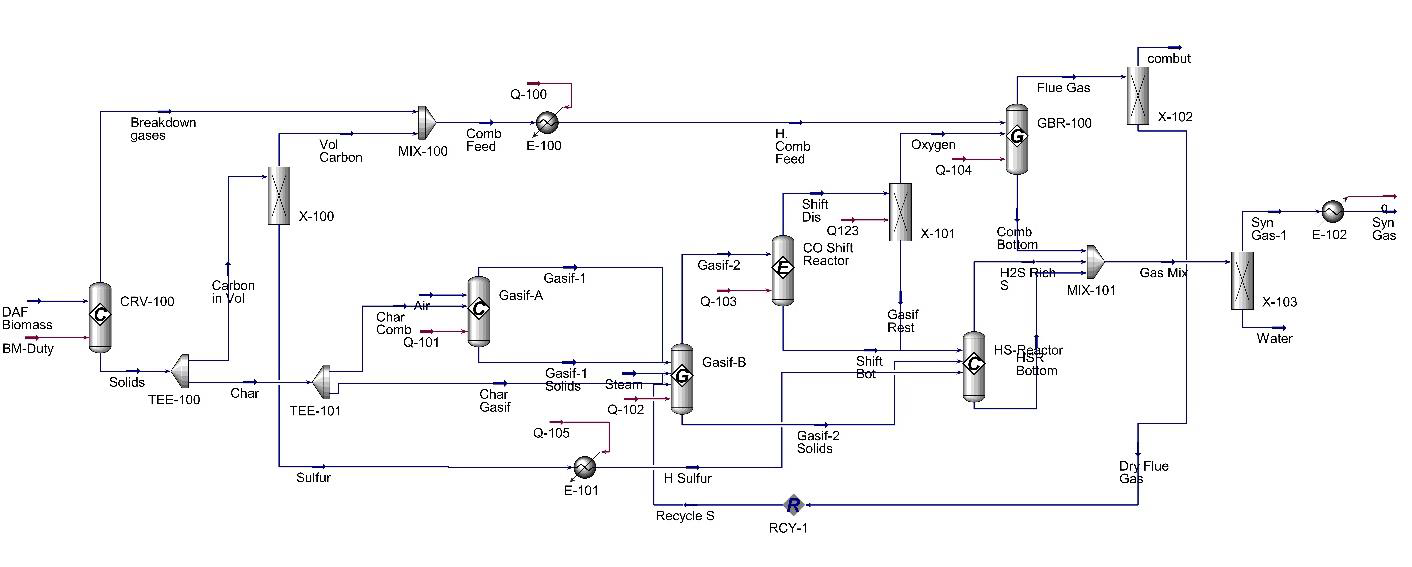
\includegraphics[width=0.98\textwidth]{figures/si/figS1_hysys_flowsheet.png}
\caption{Detailed Aspen HYSYS process-flow diagram for the integrated biomass
gasification train used to generate the \TSA{} feed. Biomass is cracked in
CRV-100, solids are split to Gasif-A and Gasif-B, heat is supplied through
the combustion loop, the CO-shift reactor tunes the \Htwo{}/CO ratio, HSR
converts sulfur to \ce{H2S}, \add{and X-103 imposes the final component split between the dry syngas
and a separate mixed-contaminant outlet labelled ``Water''.}}
\label{figS:hysys}
\end{figure}

\subsection{Feed specification and reaction network}

\add{The process-model lineage and the production-model feed
specification are distinguished here. The archived reference
configuration, Simulation~1, was used for a literature
comparison at \SI{800}{\celsius}, \SI{100}{kPa},
\SI{8}{kg.h^{-1}} biomass, \SI{16}{kg.h^{-1}} steam
and \SI{40}{kg.h^{-1}} air. The production configuration,
P-1, used the reported dry, ash-free biomass feed of
\SI{30}{kg.h^{-1}} at \SI{298}{K} and \SI{1}{bar}
and generated the syngas conditions used for adsorption
screening. Its documented reaction definitions are unchanged
from Simulation~1 except for the prescribed conversions of
R7 (20\% to 0\%) and R9 (5\% to 0\%). R1--R6 are
specified pseudo-component decomposition reactions, R10 and
R11 are equilibrium reactions based on Gibbs free energy,
and R7--R9 and R12--R13 have the tabulated conversion
specifications. These numerical conversions are prescribed
simulation inputs, not experimentally measured kinetic
constants. The model follows the reactor architecture of
\citet{Bassyouni2014DatePalmHYSYS}, but individual
conversion percentages are not taken directly from that
publication.}

\begin{table}[htbp]
\centering
\caption{Reaction definitions and prescribed conversions in
Simulation~1 and P-1, transcribed from the archived HYSYS
reaction specifications. BM is hypothetical biomass. R10 and
R11 are equilibrium reactions. The percentages of R1--R6
refer to pseudo-component conversion specifications, not
measured total gasifier conversion.}
\label{tabS:rxns}
\scriptsize
\begin{adjustbox}{max width=\textwidth}
\revtableon
\begin{tabular}{cllll}
\toprule
Rxn & Reaction & Specification & Simulation 1 & P-1 \\
\midrule
R1 & BM $\rightarrow$ 11.102 \ce{H2O} & BM conversion & 5.47\% & 5.47\% \\
R2 & BM $\rightarrow$ 16.651 C(s) & BM conversion & 55.48\% & 55.48\% \\
R3 & BM $\rightarrow$ 99.206 \ce{H2} & BM conversion & 4.53\% & 4.53\% \\
R4 & BM $\rightarrow$ 7.140 \ce{N2} & BM conversion & 0.4686\% & 0.4686\% \\
R5 & BM $\rightarrow$ 6.237 S(s) & BM conversion & 1.015\% & 1.015\% \\
R6 & BM $\rightarrow$ 6.250 \ce{O2} & BM conversion & 33.04\% & 33.04\% \\
R7 & C + $0.5$\ce{O2} $\rightarrow$ CO & C conversion & 20\% & 0\% \\
R8 & C + \ce{O2} $\rightarrow$ \ce{CO2} & C conversion & 5\% & 5\% \\
R9 & C + \ce{CO2} $\rightarrow$ 2 CO & C conversion & 5\% & 0\% \\
R10 & CO + \ce{H2O} $\rightleftharpoons$ \ce{CO2} + \ce{H2} & equilibrium & Gibbs free energy & Gibbs free energy \\
R11 & \ce{N2} + 3\ce{H2} $\rightleftharpoons$ 2\ce{NH3} & equilibrium & Gibbs free energy & Gibbs free energy \\
R12 & S + \ce{H2} $\rightarrow$ \ce{H2S} & S conversion & 100\% & 100\% \\
R13 & C + 2\ce{H2} $\rightarrow$ \ce{CH4} & C conversion & 5\% & 5\% \\
\bottomrule
\end{tabular}
\revtableoff
\end{adjustbox}
\end{table}

\subsection{\add{Reference gasification comparison and yield definitions}}
\label{secS:gas-validation}

\add{The reference configuration was compared with the
\SI{800}{\celsius} dry-product-gas composition reported
by \citet{Bassyouni2014DatePalmHYSYS}. In the archived
HYSYS export, the reference-case operating conditions were
\SI{8}{kg.h^{-1}} biomass, \SI{16}{kg.h^{-1}} steam,
\SI{40}{kg.h^{-1}} air, \SI{800}{\celsius} and
\SI{100}{kPa}. The mass-based steam-to-biomass ratio was
2.0. The literature temperature series reported by
Bassyouni et al. used a ratio of 1.5; the comparison is
therefore a near-condition consistency check rather than
an independently validated identical-condition replication.
The gas fractions were compared on the reported
hydrogen--carbon-monoxide--carbon-dioxide--methane
normalization basis.}

\begin{table}[htbp]
\centering
\caption{\add{Comparison of dry syngas composition for the
reference Simulation~1 and the \SI{800}{\celsius}
composition reported by Bassyouni et al. (2014).
Differences are signed percentage points, calculated as
Simulation~1 minus literature. Steam-to-biomass ratios
are 2.0 and 1.5, respectively.}}
\label{tabS:gas-validation}
\revtableon
\begin{tabular}{lrrr}
\toprule
Component & Literature (mol\%) & Simulation 1 (mol\%) & Difference (pp) \\
\midrule
\ce{H2} & 56.27 & 58.18 & +1.91 \\
CO       & 21.71 & 22.65 & +0.94 \\
\ce{CO2} & 18.24 & 15.70 & -2.54 \\
\ce{CH4} & 3.78 & 3.47 & -0.31 \\
\bottomrule
\end{tabular}
\revtableoff
\end{table}

\add{The reference simulation's dry syngas molar flow was
\SI{0.8644667}{kmol.h^{-1}} in the stream labelled
\texttt{Syn Gas}. The dry gas yield is defined as
\addeq{Y_{\mathrm{gas}}=\frac{\dot n_{\mathrm{dry~gas}}
V_{\mathrm{N,m}}}{\dot m_{\mathrm{biomass}}},}
where $V_{\mathrm{N,m}}=\SI{22.414}{\cubic\metre\per\kilo\mole}$
at \SI{0}{\celsius} and 1~atm. With
$\dot m_{\mathrm{biomass}}=\SI{8}{kg.h^{-1}}$,
$Y_{\mathrm{gas}}=\SI{2.422}{\cubic\metre\per\kilogram}$
(Nm\textsuperscript{3} kg\textsuperscript{-1} biomass).
The corresponding hydrogen yield, defined by
\addeq{Y_{\ce{H2}}=10^3\,\frac{\dot n_{\mathrm{dry~gas}}
y_{\ce{H2}}}{\dot m_{\mathrm{biomass}}},}
was \SI{62.87}{mol.kg^{-1}} biomass
($y_{\ce{H2}}=0.5817743$, with the factor of $10^3$
converting kmol to mol).}

\add{The model-predicted conversion of the solid-carbon feed
entering the gasification network was evaluated using
\addeq{X_{\mathrm{C,solid}}=100\left(1-
\frac{\dot m_{\mathrm{C,Gasif-2~Solids}}+
\dot m_{\mathrm{C,Comb~Bottom}}}
{\dot m_{\mathrm{C,Solids}}}\right).}
The archived HYSYS composition exports give
$\dot m_{\mathrm{C,Solids}}=
\SI{4.4384375}{kg.h^{-1}}$ and zero carbon flow
in both terminal solid outlets. Thus
$X_{\mathrm{C,solid}}=100\%$ for the specified
solid-outlet boundary. This is the predicted disappearance
of residual solid carbon under the model assumptions;
it is not the percentage of initial biomass carbon
recovered in the separated dry syngas, nor an experimental
carbon-conversion measurement.}

\add{Bassyouni et al. do not report corresponding numerical
experimental dry-gas-yield or carbon-conversion values.
For context, the distinct Fe--Ce/olivine-catalysed
pine-sawdust experiment of \citet{Liao2019PineSawdust}
reported a syngas yield of
\SI{0.93}{\cubic\metre\per\kilogram}
(Nm\textsuperscript{3} kg\textsuperscript{-1}),
$\ce{H2}$ yield of \SI{21.37}{mol.kg^{-1}},
and carbon conversion of 55.14\% at
\SI{800}{\celsius}. These experimental values are
reported as a contextual literature benchmark,
not as directly matched validation data for the
non-catalytic reference simulation; in particular, the
carbon-conversion definitions should not be assumed identical.}

\subsection{\add{Downstream component split and feed-cleanup scope}}
\label{sec:feed_cleanup}

\add{The final separation block X-103 defines the dry feed used for the
adsorption-screening calculations. It was implemented as an idealized
component split: \Htwo{}, \COtwo{}, CO and \CHfour{} are retained in
the dry ``Syn Gas-1'' stream, whereas \ce{H2O}, \Ntwo{}, \ce{H2S}
and \ce{NH3} are routed to the separate stream named ``Water''.
This outlet designation is a stream label and does not imply a
pure liquid-water condensate. In particular, the modelled removal
of \Ntwo{} is an imposed separation assumption and is not achieved
by simple water condensation.}

\add{The downstream split is documented in the archived HYSYS export.
For example, at a Gasif-2 temperature of \SI{800}{\celsius} and
steam feed of \SI{45}{kg.h^{-1}}, the reported component mass
flows in the ``Water'' outlet are shown in Table~\ref{tabS:cleanup_split}.
This illustrative point comes from a separate HYSYS sensitivity
export, not from the 20{,}301-case adsorption-screening grid.
The corresponding ``Syn Gas-1'' stream retains the four gases used
in the subsequent adsorption calculations.}

\begin{table}[htbp]
\centering
\caption{\add{Illustrative component mass flows routed to the separate
HYSYS outlet labelled ``Water'' after the idealized downstream
component split (Gasif-2 temperature: \SI{800}{\celsius}; steam feed:
\SI{45}{kg.h^{-1}}). Values are from the archived HYSYS sensitivity
export and are not measured contaminant-removal efficiencies.}}
\label{tabS:cleanup_split}
\revtableon
\begin{tabular}{lc}
\toprule
Component & Mass flow (\si{kg.h^{-1}}) \\
\midrule
\ce{H2O} & 30.3293 \\
\Ntwo{} & 31.5405 \\
\ce{H2S} & 0.3237 \\
\ce{NH3} & 0.0724 \\
\bottomrule
\end{tabular}
\revtableoff
\end{table}

\add{The model does not resolve the design, duty or removal efficiency
of individual condensation, drying, sulfur-removal, ammonia-removal
or nitrogen-separation units. Tar compounds and particulate
carryover were not represented explicitly. Practical operation
would therefore require adequate tar/particulate cleanup,
dehydration and contaminant removal before the adsorption bed;
any residual \Ntwo{} would also dilute the hydrogen-rich feed
and change the inlet partial pressures. Residual \ce{H2S},
\ce{NH3}, water or tars could introduce additional competitive
uptake, pore fouling or adsorbent-compatibility constraints not
captured in the present equilibrium model
\citep{Rey2024SyngasCleaning,Borfecchia2012HKUSTAmmonia}.}

\add{This limitation is particularly important for HKUST-1. Water
interacts strongly with its exposed Cu sites and can compete with
target gas adsorption; experimental studies have also documented
loss of crystallinity and adsorption capacity during humid
exposure or repeated hydration/dehydration cycling
\citep{AlJanabi2015HKUSTWater,Doman2019HKUSTWater}. Thus, the
predicted HKUST-1 performance and the overall adsorbent rankings
apply only to the stipulated pretreated, dry feed. Moisture
breakthrough, realistic contaminant-removal efficiencies and
adsorbent lifetime were not modelled.}

\subsection{Base-case stream data}

\begin{table}[htbp]
\centering
\caption{Simulated dry syngas composition leaving X-103 in the base case.
Conditions: \SI{298}{K}, \SI{1}{bar}; total mass flow =
\SI{34.55325}{kg.h^{-1}}.}
\label{tabS:molefrac}
\begin{tabular}{lc}
\toprule
Component & Mole fraction \\
\midrule
\Htwo{} & 0.6716 \\
\COtwo{} & 0.3172 \\
CO & 0.0111 \\
\CHfour{} & $2.3769\times 10^{-5}$ \\
C, \Ntwo, S-amorphous, \ce{O2}, \ce{H2O}, \ce{NH3}, \ce{H2S}, BM* & 0.0000 \\
\textbf{Total} & \textbf{1.0000} \\
\bottomrule
\end{tabular}
\end{table}

\begin{table}[htbp]
\centering
\caption{Corresponding base-case component mass flow rates.}
\label{tabS:massflow}
\begin{tabular}{lc}
\toprule
Component & Mass flow (\si{kg.h^{-1}}) \\
\midrule
\Htwo{} & 2.9934 \\
\COtwo{} & 30.8686 \\
CO & 0.6904 \\
\CHfour{} & 0.0008 \\
Others & 0.0000 \\
\textbf{Total} & \textbf{34.55325} \\
\bottomrule
\end{tabular}
\end{table}

\add{The zero values reported for other components in the dry syngas
tables refer to the assumed post-X-103 adsorption inlet; they do
not imply that \ce{H2O}, \Ntwo{}, \ce{H2S} or \ce{NH3} were absent
from the upstream gasification process. Their separate outlet
flows are illustrated in Table~\ref{tabS:cleanup_split}.}

\FloatBarrier
\section{Upstream sensitivity maps}

Increasing steam raises the \Htwo{} fraction and suppresses CO and \CHfour{},
producing a more \COtwo-rich feed. Increasing temperature at fixed steam
further promotes reforming and eliminates most methane. These trends define
the feed-composition regimes used in the main-text adsorbent comparison:
low-steam/high-temperature operation favours higher hydrogen with residual
CO, while high-steam operation pushes the separation problem toward
\COtwo-rich, methane-poor feeds.

\begin{figure}[htbp]
\centering
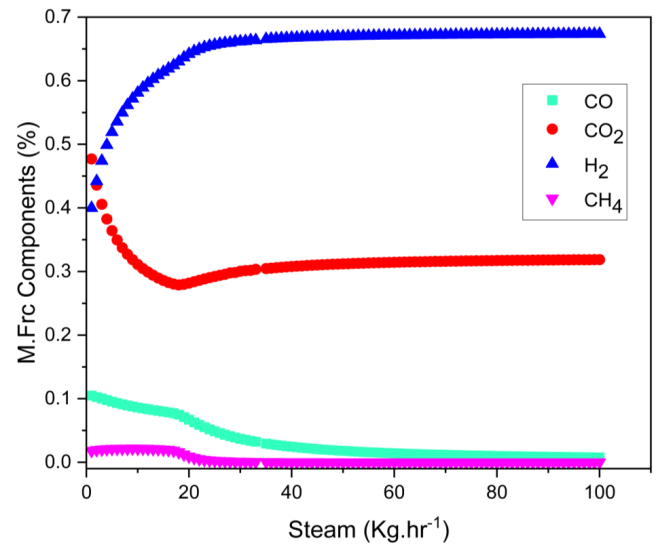
\includegraphics[width=0.82\textwidth]{figures/si/figS2_steam_composition.png}
\caption{Steam sensitivity of dry syngas composition. Increasing steam changes
the mole fractions of \Htwo{}, \COtwo{}, CO and \CHfour{}, supporting the
main-text conclusion that steam addition suppresses CO and \CHfour{} but drives
the feed toward a more \COtwo-rich separation problem.}
\label{figS:steamx}
\end{figure}

\begin{figure}[htbp]
\centering
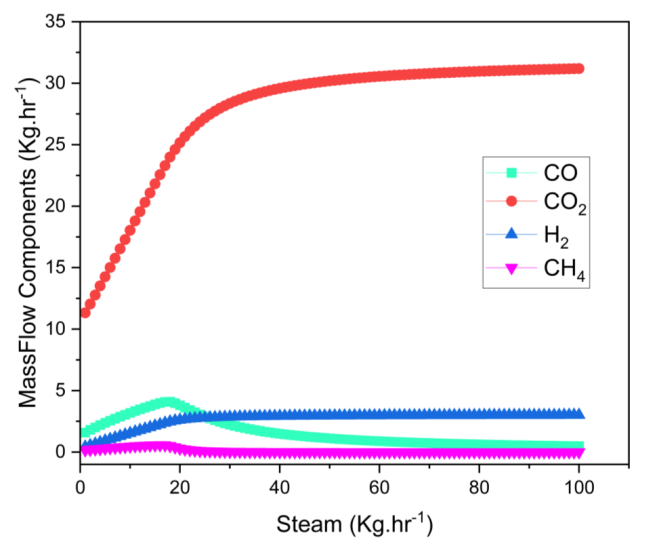
\includegraphics[width=0.82\textwidth]{figures/si/figS3_steam_mass_flow.png}
\caption{Steam sensitivity of component mass flow rates. Composition trends
in \Cref{figS:steamx} correspond to real changes in component flow rather
than dilution effects alone.}
\label{figS:steamm}
\end{figure}

\begin{figure}[htbp]
\centering
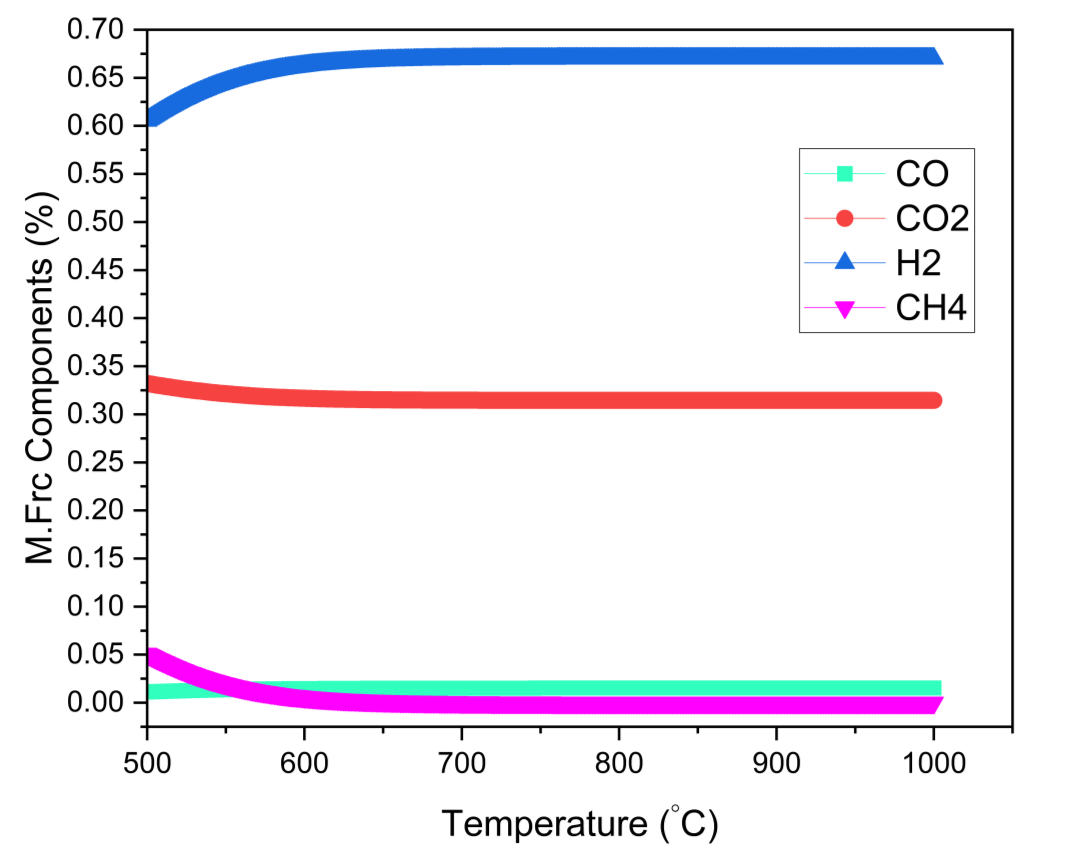
\includegraphics[width=0.82\textwidth]{figures/si/figS4_temperature_composition.png}
\caption{Temperature sensitivity of dry syngas composition at fixed steam
feed. Higher temperature promotes hydrogen-rich reforming/gasification
behaviour and suppresses methane, defining the high-temperature feed regime
used in the main-text material comparison.}
\label{figS:tempx}
\end{figure}

\begin{figure}[htbp]
\centering
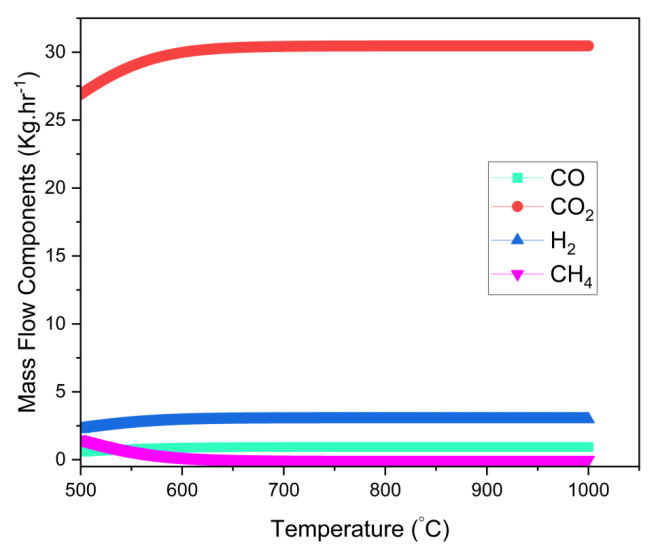
\includegraphics[width=0.82\textwidth]{figures/si/figS5_temperature_mass_flow.png}
\caption{Temperature sensitivity of component mass flow rates at fixed steam
feed. Temperature changes the amount of feed to be treated and the impurity
mix entering the \TSA{} unit.}
\label{figS:tempm}
\end{figure}

\FloatBarrier
\section{Adsorption model equations}

For a single component, the one-site Langmuir loading is
\begin{equation}
q_i = \frac{q_i^{\mathrm{sat}} b_i p_i}{1+b_i p_i}.
\label{eqS:langmuir}
\end{equation}

For a mixture, the extended Langmuir form is
\begin{equation}
q_i = \frac{q_i^{\mathrm{sat}} b_i p_i}{1+\sum_j b_j p_j}.
\label{eqS:extended}
\end{equation}

The affinity parameter uses an Arrhenius-like relation,
\begin{equation}
b_i(T)=b_{0,i}\exp\left(-\frac{\Delta H_i}{RT}\right),
\label{eqS:arrhenius}
\end{equation}
with fitted pre-exponential term $b_{0,i}$ and apparent adsorption enthalpy
parameter $\Delta H_i$.

\add{In the primary \TSA{} screening calculation, the adsorption temperature
is fixed at $T_{\mathrm{ads}}=\SI{298}{K}$, while the regeneration
(or desorption) temperature $T_{\mathrm{des}}$ takes one of ten
set-points: \SI{313.2}{K}, \SI{328.4}{K}, \SI{343.6}{K},
\SI{358.8}{K}, \SI{374}{K}, \SI{389.2}{K}, \SI{404.4}{K},
\SI{419.6}{K}, \SI{434.8}{K} and \SI{450}{K}. Accordingly, the
\TSA{} thermal set-point is $T_{\mathrm{des}}$, and the thermal swing
width in the working-capacity and regeneration-energy expressions is
$T_{\mathrm{des}}-T_{\mathrm{ads}}$. The primary \TSA{} scoring uses an
adsorption pressure of \SI{1}{bar}.}

The working capacity for impurity $i$ is
\begin{equation}
\Delta q_i = q_i(T_{\mathrm{ads}},p_i)-q_i(T_{\mathrm{des}},p_i),
\label{eqS:working_capacity}
\end{equation}
and the adsorbent mass requirement used in the inventory-scaling analysis is
\begin{equation}
m_{\mathrm{ads},i}=\frac{n_{i,\mathrm{feed}}\eta_i}{\Delta q_i}, \qquad
m_{\mathrm{ads,max}}=\max_i(m_{\mathrm{ads},i}),
\label{eqS:mads}
\end{equation}
with $i\in\{\COtwo,\mathrm{CO},\CHfour\}$. Throughout, $m_{\mathrm{ads}}$
denotes total dry adsorbent mass and applies to HKUST-1, Cu-TDPAT and
Zeolite~13X on the same normalisation.

Hydrogen productivity for \TSA{} is
\begin{equation}
\Pi_{\Htwo}=\frac{n_{\Htwo,\mathrm{out}}}{m_{\mathrm{ads}}t_{\mathrm{cycle}}},
\label{eqS:prod}
\end{equation}
with $t_{\mathrm{cycle}}=\SI{900}{s}$ throughout the manuscript and Supporting
Information.

The specific regeneration energy per unit hydrogen produced combines the
sensible heating of the controlling adsorbent inventory over the thermal
swing window with the enthalpy required to desorb the retained impurities:
\begin{equation}
E_{\mathrm{reg}} = \frac{
  m_{\mathrm{ads,max}} \, C_{p,\mathrm{ads}} \, (T_{\mathrm{des}} - T_{\mathrm{ads}})
  + \sum_i q_{i,\mathrm{ads}} \, m_{\mathrm{ads,max}} \, (-\Delta H_i)
}{
  n_{\Htwo,\mathrm{out}}
},
\label{eqS:ereg}
\end{equation}
where $C_{p,\mathrm{ads}}$ is the mass-specific adsorbent heat capacity,
$T_{\mathrm{des}} - T_{\mathrm{ads}}$ is the thermal swing width,
$q_{i,\mathrm{ads}}$ is the equilibrium loading of impurity $i$ at
adsorption conditions, and $-\Delta H_i$ is the adsorption enthalpy of
species $i$. In the reproduction-code basis, $m_{\mathrm{ads,max}}$ is in kg,
$q_i$ is in mol kg$^{-1}$ and $-\Delta H_i$ is in kJ mol$^{-1}$, so the
adsorbed-phase enthalpy term is obtained on a kJ basis. The solid adsorbent
heat capacities used for the MOF sensible-heat term are $C_p=0.7$ kJ kg$^{-1}$
K$^{-1}$ for HKUST-1 and $C_p=0.92$ kJ kg$^{-1}$ K$^{-1}$ for Cu-TDPAT. The
component-wise heat-capacity values retained in \Cref{tabS:zeolite13x_params}
are kept in the same source-parameter basis used for the Zeolite~13X scoring. Because Eq.~\eqref{eqS:ereg}
does not include bed hardware, heat losses, heat-front dynamics, compressor
work or vacuum-pump work, $E_{\mathrm{reg}}$ is used as a consistent
comparative screening score rather than as an absolute plant heat-duty design
value.

\FloatBarrier
\section{Langmuir parameters for HKUST-1 and Cu-TDPAT}

\begin{table}[htbp]
\centering
\caption{HKUST-1 temperature-specific single-component Langmuir fits.}
\label{tabS:hkustfit}
\small
\begin{adjustbox}{max width=\textwidth}
\begin{tabular}{ccccc}
\toprule
$T$ (K) & Gas & $q^{\mathrm{sat}}$ (mmol g$^{-1}$) & $b$ (bar$^{-1}$) & $R^2$ \\
\midrule
295 & CO & -- & 0.130792 & 0.999918 \\
318 & CO & 9.9522 & 0.076456 & 0.999924 \\
353 & CO & -- & 0.031261 & 0.999956 \\
295 & \COtwo{} & -- & 0.546887 & 0.999999 \\
318 & \COtwo{} & 16.65645 & 0.285902 & 0.999971 \\
353 & \COtwo{} & -- & 0.097758 & 0.999960 \\
295 & \CHfour{} & -- & 0.096682 & 0.999999 \\
318 & \CHfour{} & 12.31266 & 0.058688 & 0.999986 \\
353 & \CHfour{} & -- & 0.027059 & 0.999995 \\
\bottomrule
\end{tabular}
\end{adjustbox}
\end{table}

\begin{table}[htbp]
\centering
\caption{HKUST-1 temperature-dependence parameters. Adsorbent heat capacity
used in the regeneration-energy calculation (Eq.~\eqref{eqS:ereg}):
$C_p = 0.7$ kJ kg$^{-1}$ K$^{-1}$.}
\label{tabS:hkustarr}
\small
\begin{adjustbox}{max width=\textwidth}
\begin{tabular}{ccccc}
\toprule
Gas & $q^{\mathrm{sat}}$ (mmol g$^{-1}$) & $b_0$ & $-\Delta H/R$ & $R^2$ \\
\midrule
CO & 9.9522 & $2.13384\times10^{-5}$ & -21.4742 & 0.9945 \\
\COtwo{} & 16.65645 & $1.51881\times10^{-5}$ & -25.8299 & 0.9948 \\
\CHfour{} & 12.31266 & $4.13681\times10^{-5}$ & -19.0815 & 0.9970 \\
\bottomrule
\end{tabular}
\end{adjustbox}
\end{table}

\begin{table}[htbp]
\centering
\caption{Cu-TDPAT temperature-specific single-component Langmuir fits.}
\label{tabS:cutdpatfit}
\small
\begin{adjustbox}{max width=\textwidth}
\begin{tabular}{ccccc}
\toprule
$T$ (K) & Gas & $q^{\mathrm{sat}}$ (mmol g$^{-1}$) & $b$ (bar$^{-1}$) & $R^2$ \\
\midrule
288.15 & CO & -- & 0.611346 & 0.999141 \\
298.15 & CO & 3.859979 & 0.428403 & 0.999126 \\
308.15 & CO & -- & 0.307217 & 0.999249 \\
288.15 & \COtwo{} & -- & 1.719113 & 1.000000 \\
298.15 & \COtwo{} & 9.311152 & 1.168312 & 1.000000 \\
308.15 & \COtwo{} & -- & 0.847821 & 1.000000 \\
288.15 & \CHfour{} & -- & 0.196846 & 0.999893 \\
298.15 & \CHfour{} & 8.990616 & 0.151619 & 0.999886 \\
308.15 & \CHfour{} & -- & 0.118924 & 0.999881 \\
\bottomrule
\end{tabular}
\end{adjustbox}
\end{table}

\begin{table}[htbp]
\centering
\caption{Cu-TDPAT temperature-dependence parameters. Adsorbent heat capacity
used in the regeneration-energy calculation (Eq.~\eqref{eqS:ereg}):
$C_p = 0.92$ kJ kg$^{-1}$ K$^{-1}$.}
\label{tabS:cutdpatarr}
\small
\begin{adjustbox}{max width=\textwidth}
\begin{tabular}{ccccc}
\toprule
Gas & $q^{\mathrm{sat}}$ (mmol g$^{-1}$) & $b_0$ & $-\Delta H/R$ & $R^2$ \\
\midrule
CO       & 3.859979 & $1.31907\times10^{-5}$ & -26.018663 & 1.0000 \\
\COtwo{} & 9.311152 & $3.1548\times10^{-5}$  & -26.110117 & 0.9988 \\
\CHfour{} & 8.990616 & $8.35471\times10^{-5}$ & -18.6017436 & 1.0000 \\
\bottomrule
\end{tabular}
\end{adjustbox}
\end{table}

\FloatBarrier
\section{Zeolite~13X isotherm parameters}
\label{secS:zeolite13x}

Zeolite~13X exhibits pronounced surface heterogeneity due to its
cation-exchange sites, and its single-component isotherms for CO,
\COtwo{}, and \CHfour{} are represented by the three-parameter
temperature-dependent Sips isotherm \citep{Ruthven1984PSA}:
\begin{equation}
q_i = \frac{q_i^{\mathrm{sat}}(T) \, K_i(T) \, p_i^{\,s_i(T)}}
     {1 + K_i(T) \, p_i^{\,s_i(T)}},
\label{eqS:sips13x}
\end{equation}
with temperature-dependent saturation capacity, affinity, and
heterogeneity parameter:
\begin{align}
q_i^{\mathrm{sat}}(T) &= a_i + b_i \, T, \label{eqS:sipsqsat}\\
K_i(T) &= A_i \, \exp\!\left(\frac{B_i}{T}\right), \label{eqS:sipsK}\\
s_i(T) &= \alpha_i + \frac{\beta_i}{T}. \label{eqS:sipss}
\end{align}
The mixture form uses the analogous multi-Sips convention:
\begin{equation}
q_i = \frac{q_i^{\mathrm{sat}}(T) \, K_i(T) \, p_i^{\,s_i(T)}}
     {1 + \sum_j K_j(T) \, p_j^{\,s_j(T)}}.
\label{eqS:sips_mixture}
\end{equation}
The heterogeneity parameter $s_i$ approaches unity in the homogeneous-surface
limit, where Eq.~\eqref{eqS:sips13x} reduces to the Langmuir form used for
the MOFs (Eq.~\eqref{eqS:langmuir}). For Zeolite~13X, fitted $s_i$ values
deviate meaningfully from unity, justifying the Sips extension for this
heterogeneous aluminosilicate framework.

Parameters used in the scoring calculation (\Cref{tabS:zeolite13x_params})
were taken from the single-component isotherm measurements of Park et
al.~\citep{Park2016Zeolite13X}, as tabulated and used in the VPSA modelling
work of Streb and Mazzotti~\citep{Streb2020VPSAH2CO2}. Adsorption energies
$-\Delta U_i$ used in the regeneration-energy calculation
(Eq.~\eqref{eqS:ereg}) are from the same reference.

\begin{table}[htbp]
\centering
\caption{Zeolite~13X temperature-dependent Sips parameters used in the
scoring calculation. From Park et al.~\citep{Park2016Zeolite13X},
tabulated as in Streb and Mazzotti~\citep{Streb2020VPSAH2CO2}. Affinity
constants converted from kPa$^{-1}$ to bar$^{-1}$ ($A_i^{\mathrm{bar}} =
A_i^{\mathrm{kPa}} \times 100$).}
\label{tabS:zeolite13x_params}
\small
\begin{adjustbox}{max width=\textwidth}
\begin{tabular}{ccccccccc}
\toprule
Component &
$C_p$ (kJ mol$^{-1}$ K$^{-1}$) &
$a_i$ (mol kg$^{-1}$) &
$b_i \times 10^{3}$ (mol kg$^{-1}$ K$^{-1}$) &
$A_i \times 10^{4}$ (bar$^{-1}$) &
$B_i$ (K) &
$\alpha_i \times 10^{2}$ &
$\beta_i$ (K) &
$-\Delta U_i$ (kJ mol$^{-1}$) \\
\midrule
CO      & 0.02915 &  9.614 & $-19.27$ & 13.95 & 1496 & $-14.61$ & 407   & 25 \\
\COtwo{} & 0.03735 &  8.984 & $-9.867$ &  2.266 & 3130 &  36.22   & 454.4 & 37 \\
\CHfour{} & 0.0358  & 13.69  & $-31.67$ & 38.36 & 1083 &  66.51   &  97.8 & 19 \\
\bottomrule
\end{tabular}
\end{adjustbox}
\end{table}

\FloatBarrier
\section{Isotherms and working-capacity figures}

Across both MOFs, \COtwo{} dominates equilibrium uptake and working capacity.
CO and \CHfour{} remain much smaller under the low-pressure conditions
relevant to the \TSA{} feed, but they remain process-relevant because even
small changes in CO or \CHfour{} alter competitive site occupation and
material ranking.

\begin{figure}[htbp]
\centering
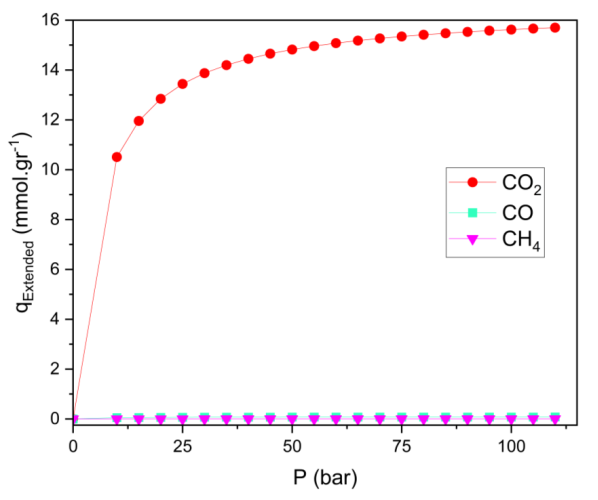
\includegraphics[width=0.82\textwidth]{figures/si/figS6_hkust_isotherm_295K.png}
\caption{HKUST-1 extended isotherms at \SI{295}{K}. \COtwo{} rises steeply
and dominates uptake, whereas CO and \CHfour{} remain comparatively small,
supporting the impurity-retention interpretation in the main text.}
\label{figS:hkust295}
\end{figure}

\begin{figure}[htbp]
\centering
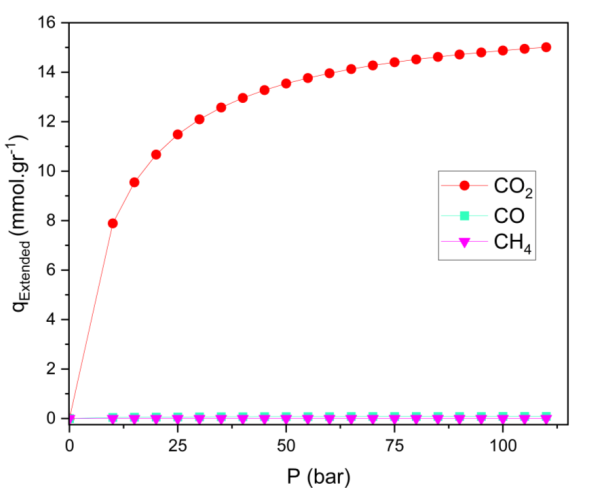
\includegraphics[width=0.82\textwidth]{figures/si/figS7_hkust_isotherm_318K.png}
\caption{HKUST-1 extended isotherms at \SI{318}{K}. The \COtwo{} curve
remains dominant but flattens relative to \SI{295}{K}, demonstrating the
thermal sensitivity that enables \TSA{} regeneration.}
\label{figS:hkust318}
\end{figure}

\begin{figure}[htbp]
\centering
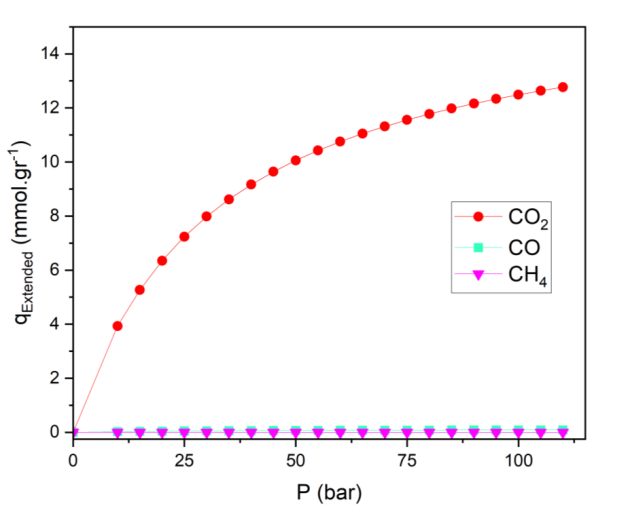
\includegraphics[width=0.82\textwidth]{figures/si/figS8_hkust_isotherm_353K.png}
\caption{HKUST-1 extended isotherms at \SI{353}{K}. \COtwo{} capacity
decreases further while CO and \CHfour{} remain small, showing why
high-temperature desorption reduces impurity inventory.}
\label{figS:hkust353}
\end{figure}

\begin{figure}[htbp]
\centering
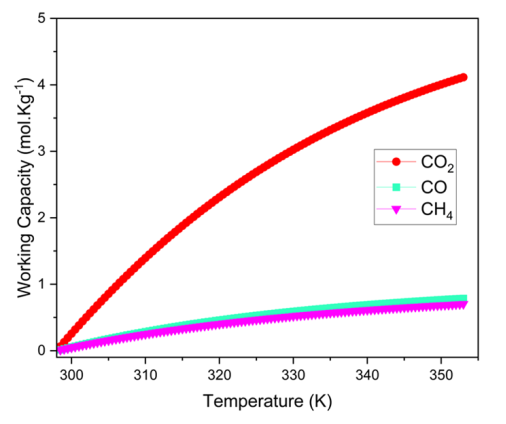
\includegraphics[width=0.82\textwidth]{figures/si/figS9_hkust_working_capacity.png}
\caption{HKUST-1 working capacities for \COtwo{}, CO and \CHfour{} across
the \TSA{} temperature window. \COtwo{} working capacity dominates the
heat-regeneration problem, while CO and \CHfour{} remain smaller but still
trigger regime-dependent ranking changes.}
\label{figS:hkustwc}
\end{figure}

\begin{figure}[htbp]
\centering
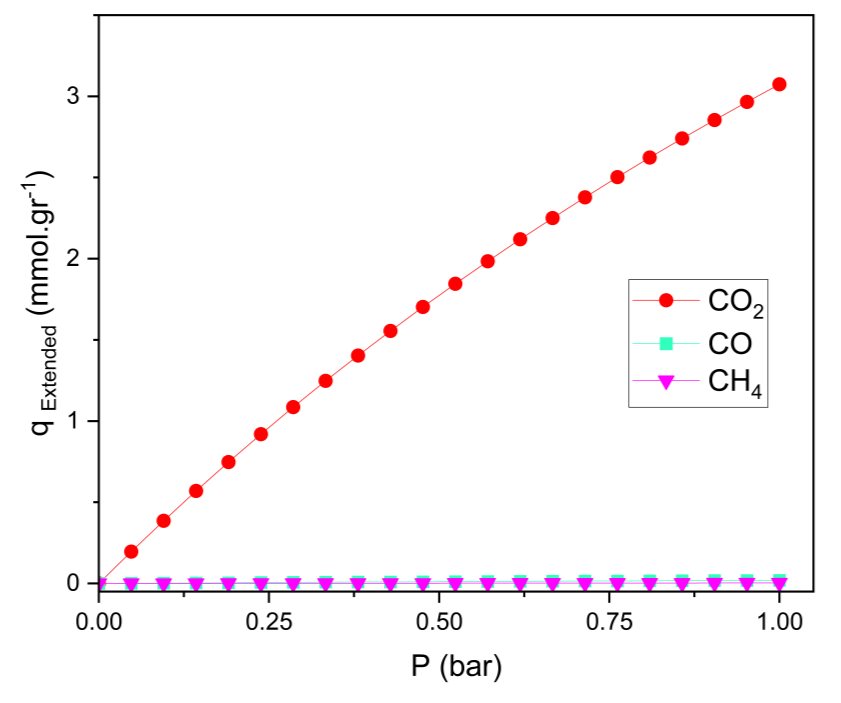
\includegraphics[width=0.82\textwidth]{figures/si/figS10_cutdpat_isotherm_288K.png}
\caption{Cu-TDPAT extended isotherms at \SI{288.15}{K}. Lower absolute
\COtwo{} capacity than HKUST-1 combined with weak CO and \CHfour{} loadings
is consistent with Cu-TDPAT acting as a flexible MOF comparator rather than
as a maximum-capacity material.}
\label{figS:cutdpat288}
\end{figure}

\begin{figure}[htbp]
\centering
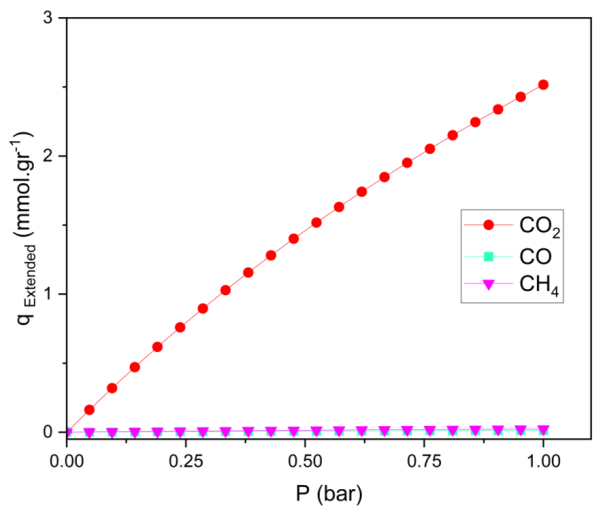
\includegraphics[width=0.82\textwidth]{figures/si/figS11_cutdpat_isotherm_298K.png}
\caption{Cu-TDPAT extended isotherms at \SI{298.15}{K}. \COtwo{} remains the
dominant impurity while CO and \CHfour{} contribute weak but process-relevant
competition.}
\label{figS:cutdpat298}
\end{figure}

\begin{figure}[htbp]
\centering
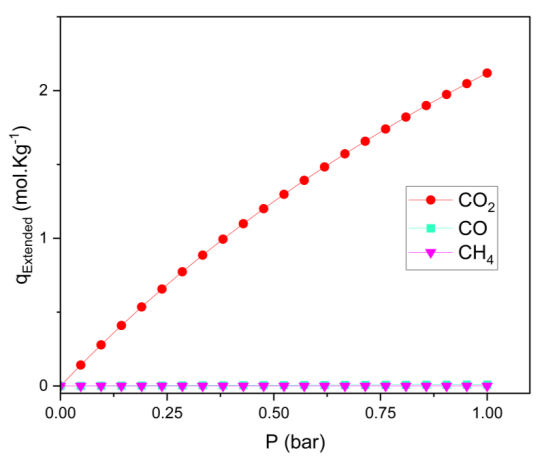
\includegraphics[width=0.82\textwidth]{figures/si/figS12_cutdpat_isotherm_308K.png}
\caption{Cu-TDPAT extended isotherms at \SI{308.15}{K}. Raising temperature
lowers absolute impurity loading and illustrates why thermal set-point
control makes this MOF competitive in selected regimes.}
\label{figS:cutdpat308}
\end{figure}

\begin{figure}[htbp]
\centering
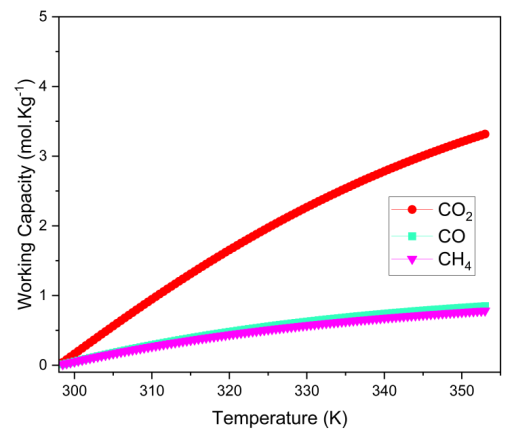
\includegraphics[width=0.82\textwidth]{figures/si/figS13_cutdpat_working_capacity.png}
\caption{Cu-TDPAT working capacities for \COtwo{}, CO and \CHfour{} across
the \TSA{} temperature window. Cu-TDPAT can be process-flexible, but its
energy penalty rises when \COtwo{} regeneration dominates.}
\label{figS:cutdpatwc}
\end{figure}

\begin{figure}[htbp]
\centering
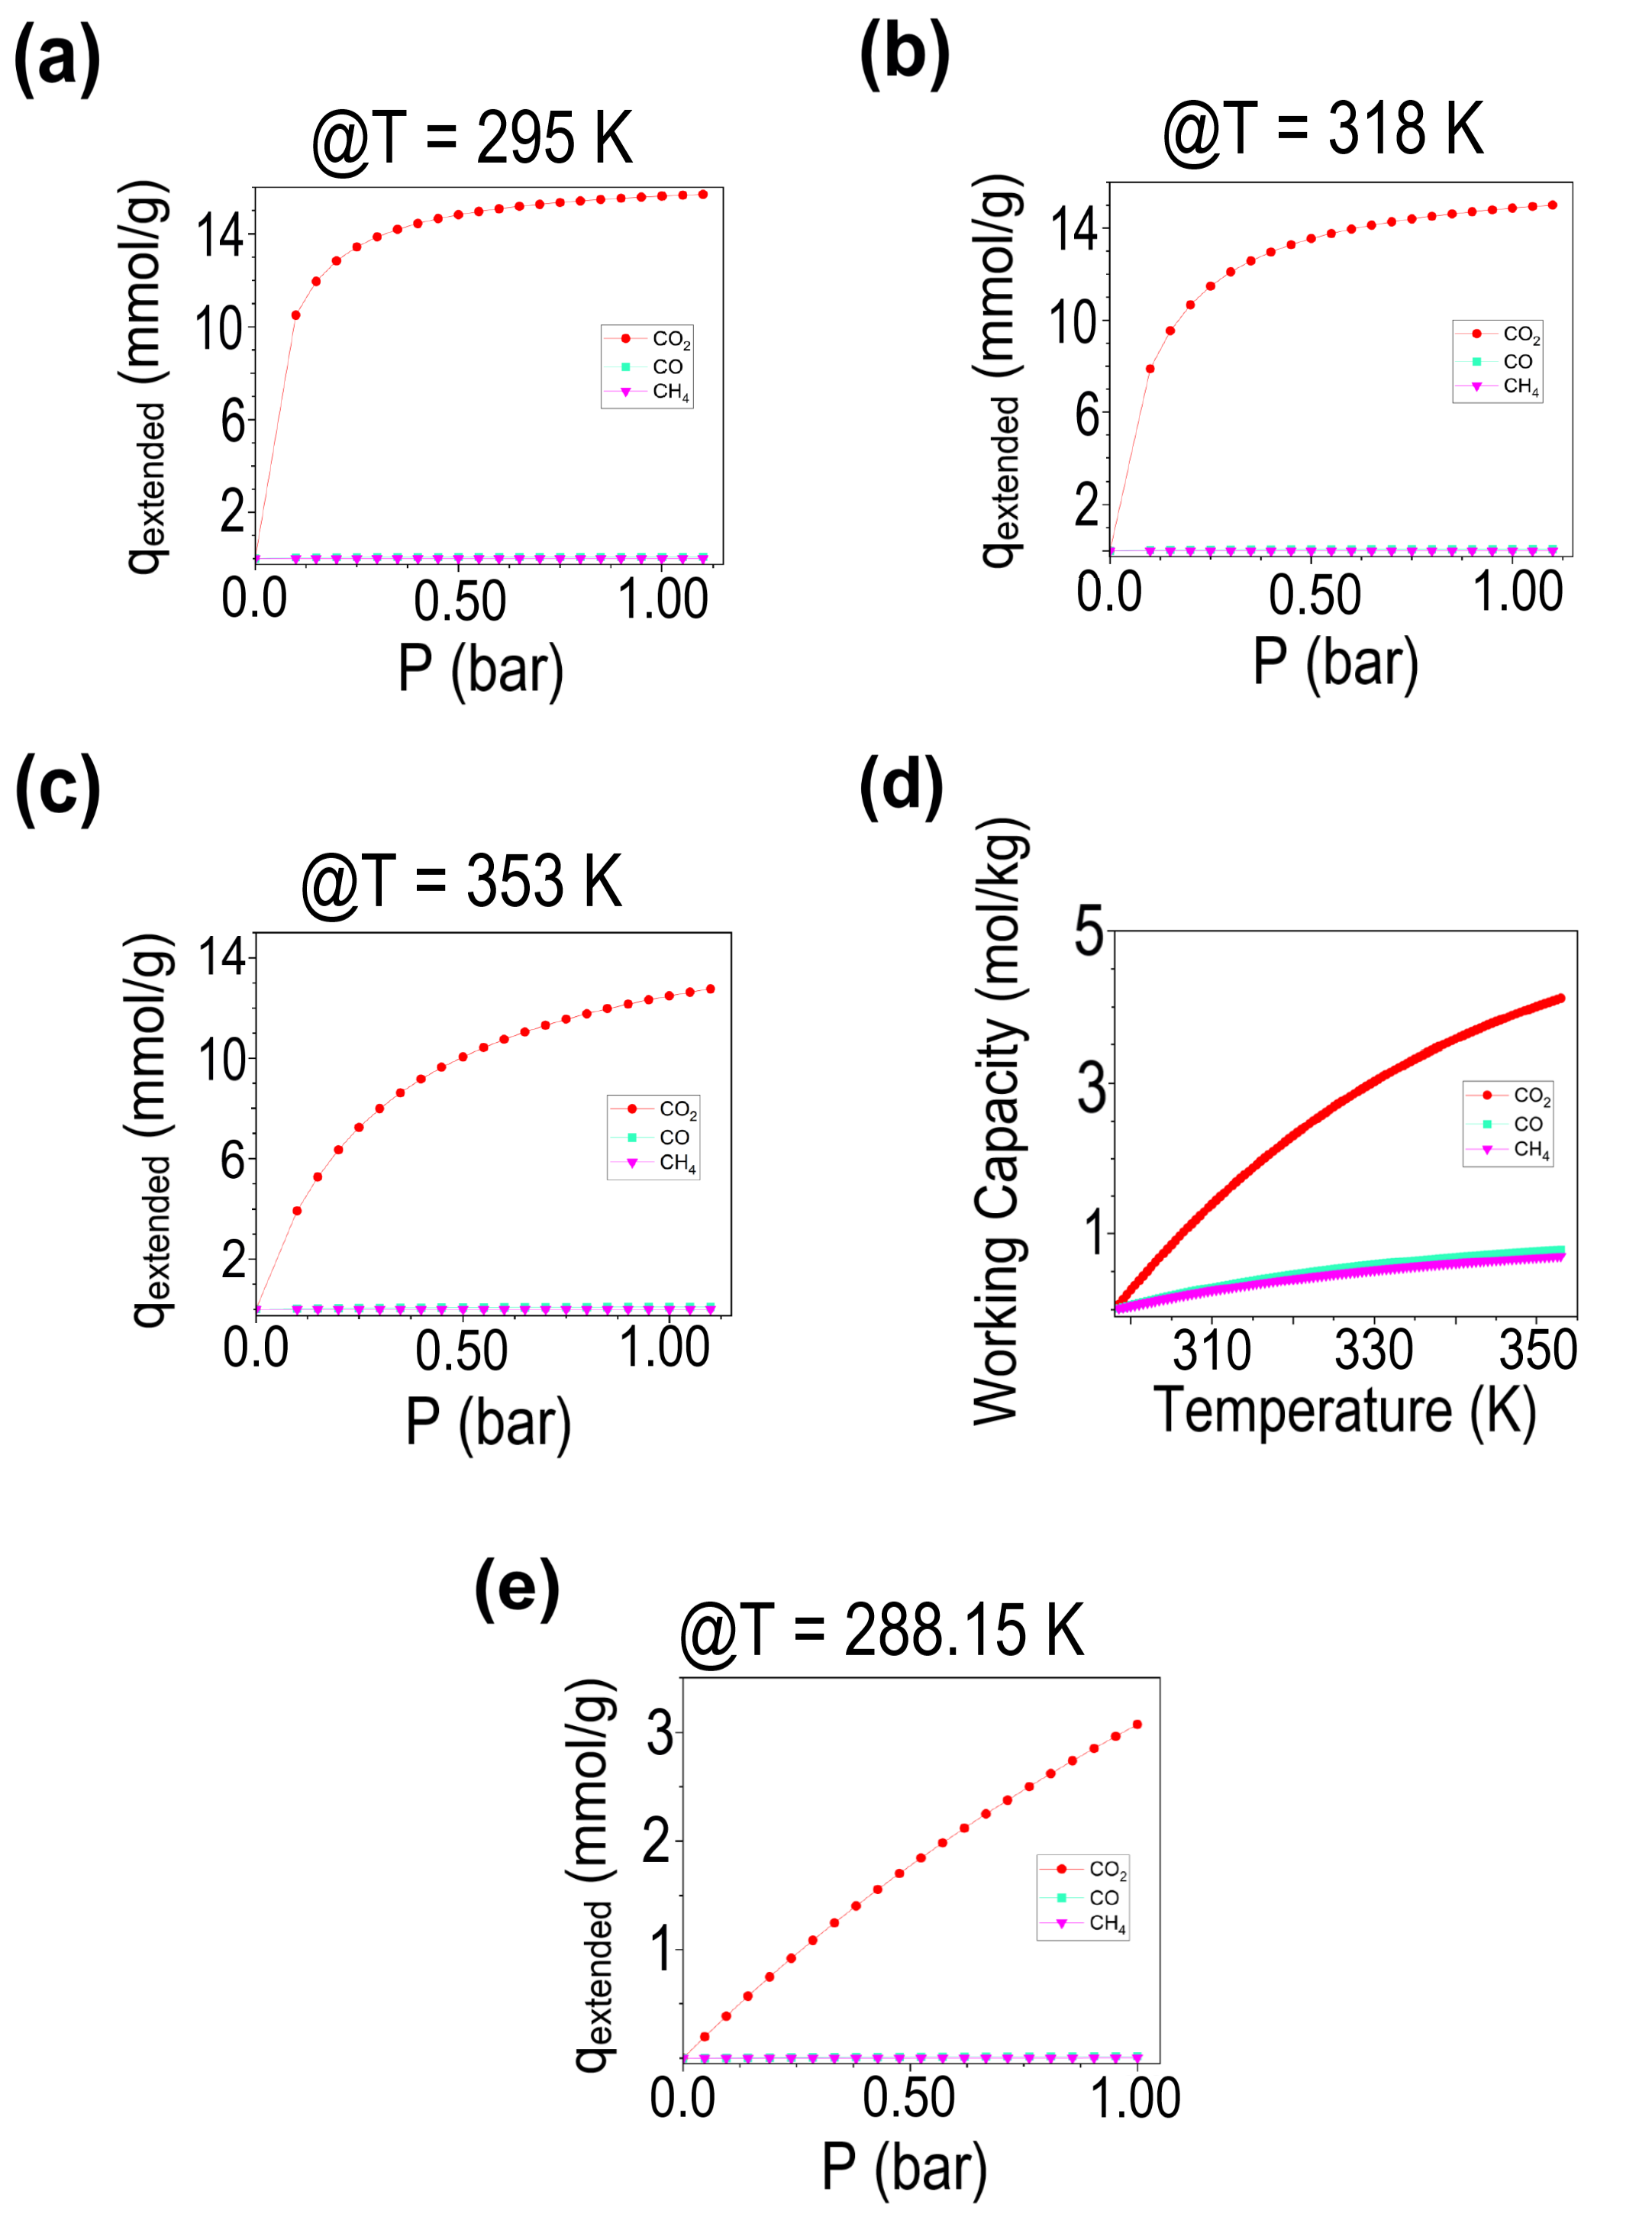
\includegraphics[width=0.78\textwidth]{figures/si/figS14_impurity_isotherms_working_capacity.png}
\caption{Composite adsorption-thermodynamics panel supporting the main-text
discussion of regime-dependent material selection. Panels (a--c) show HKUST-1
extended isotherms for \COtwo{}, CO and \CHfour{} at (a) \SI{295}{K},
(b) \SI{318}{K} and (c) \SI{353}{K}; panel (d) reports the corresponding
HKUST-1 working capacities across the \TSA{} temperature window; panel (e)
shows the Cu-TDPAT isotherm at \SI{288.15}{K}. Dominant \COtwo{} uptake
explains why regeneration energy is often \COtwo-controlled, while smaller
CO and \CHfour{} loadings explain why these species act mainly as
regime-switching impurities.}
\label{figS:main_isotherms}
\end{figure}

\FloatBarrier
\section{Metric scope and cycle-time consistency}

All productivity values used in the main text are based on the standardised
\TSA{} cycle time defined in Eq.~\eqref{eqS:prod},
$t_{\mathrm{cycle}}=\SI{900}{s}$. Earlier base-case summary tables that used
different cycle assumptions were not used as the basis for the main-text
regime maps or material-selection conclusions. The manuscript instead
emphasises the full atlas of 609{,}030 process--material scoring rows
(20{,}301 gasifier scenarios $\times$ 10 \TSA{} thermal set-points $\times$
3 adsorbents), where productivity, regeneration energy and
adsorbent-inventory metrics are evaluated consistently across HKUST-1,
Cu-TDPAT and Zeolite~13X.

\FloatBarrier
\section{Tree-ensemble surrogate, held-out performance, and TreeSHAP attribution}
\label{secS:xgb}

A tree-ensemble surrogate was used as an attribution layer over the computed
process--material atlas. Its purpose was to reproduce the computed response
surface using controllable variables only and to support exact TreeSHAP
feature attribution, not to replace the equilibrium \TSA{} scoring model or
to predict performance for unstudied adsorbents.

\subsection{Inputs, outputs and rationale for excluding composition variables}

The surrogate inputs were steam mass flow, gasifier temperature, \TSA{}
thermal set-point and one-hot adsorbent identity (\Cref{tabS:xgbio}). Syngas
mole fractions and product molar flow were excluded because they are outputs
of the gasifier simulation and therefore mediate the effect of the upstream
gasifier set-points on the \TSA{} scoring. Including both the gasifier
set-points and their downstream composition consequences in a single
attribution model would mix upstream causes with intermediate variables and
make the attribution ambiguous. The composition variables are analysed
directly through the gasifier maps in Figure~3 of the main manuscript; the
surrogate attribution is restricted to controllable process/material variables.

The five response variables were adsorbent mass controlled by \CHfour{}
($m_{\mathrm{ads},\CHfour}$), adsorbent mass controlled by CO
($m_{\mathrm{ads},\mathrm{CO}}$), adsorbent mass controlled by \COtwo{}
($m_{\mathrm{ads},\COtwo}$), hydrogen productivity ($\Pi_{\Htwo}$), and
regeneration energy consumption ($E_{\mathrm{reg}}$).

\begin{table}[htbp]
\centering
\caption{Inputs and outputs of the tree-ensemble surrogate.}
\label{tabS:xgbio}
\small
\begin{adjustbox}{max width=\textwidth}
\begin{tabular}{lll}
\toprule
Symbol/label & Unit & Role \\
\midrule
\multicolumn{3}{l}{\textit{Inputs (controllable variables only)}} \\
Steam mass flow & \si{kg.h^{-1}} & Upstream gasifier control variable \\
Gasifier temperature & \si{\celsius} & Upstream gasifier control variable \\
\TSA{} thermal set-point & K & Downstream separation control variable \\
Adsorbent identity (HKUST-1) & 0/1 & One-hot indicator \\
Adsorbent identity (Cu-TDPAT) & 0/1 & One-hot indicator \\
Adsorbent identity (Zeolite~13X) & 0/1 & One-hot indicator \\
\midrule
\multicolumn{3}{l}{\textit{Excluded inputs (downstream mediators)}} \\
\Htwo{} mole fraction & mol/mol & Output of the gasifier model \\
\COtwo{} mole fraction & mol/mol & Output of the gasifier model \\
CO mole fraction & mol/mol & Output of the gasifier model \\
\CHfour{} mole fraction & mol/mol & Output of the gasifier model \\
Product molar flow & kmol/h & Output of the gasifier model \\
\midrule
\multicolumn{3}{l}{\textit{Outputs (screening metrics)}} \\
$m_{\mathrm{ads},\CHfour}$ & kg & Adsorbent mass required when \CHfour{} controls breakthrough \\
$m_{\mathrm{ads},\mathrm{CO}}$ & kg & Adsorbent mass required when CO controls breakthrough \\
$m_{\mathrm{ads},\COtwo}$ & kg & Adsorbent mass required when \COtwo{} controls breakthrough \\
$\Pi_{\Htwo}$ & mol H$_2$ kg$^{-1}$ h$^{-1}$ & Specific hydrogen productivity \\
$E_{\mathrm{reg}}$ & MJ kg$^{-1}$ H$_2$ & Regeneration energy per unit hydrogen recovered \\
\bottomrule
\end{tabular}
\end{adjustbox}
\end{table}

\subsection{Model and split protocol}

Separate XGBoost regressors were trained for each response variable using
the hyperparameters in \Cref{tabS:xgbparams}. Two held-out protocols were
used. The random-row split tests interpolation over the full scenario table.
The gasifier-scenario-grouped split holds out entire gasifier scenarios so
that no row associated with a held-out gasifier condition appears during
training. The grouped split is the more conservative test of whether the
surrogate reproduces the atlas across unseen gasifier operating points. In
both protocols 15\% of the data was held out.

\begin{table}[htbp]
\centering
\caption{XGBoost hyperparameters used for the tree-ensemble surrogate.}
\label{tabS:xgbparams}
\small
\begin{tabular}{lc}
\toprule
Hyperparameter & Value \\
\midrule
Number of estimators & 600 \\
Maximum tree depth & 5 \\
Learning rate & 0.04 \\
Subsample fraction & 0.85 \\
Column sample by tree & 0.85 \\
Objective & squared-error regression \\
Tree method & histogram \\
Regularisation $\lambda$ & 1.0 \\
Regularisation $\alpha$ & 0.0 \\
Random seed & 442 \\
\bottomrule
\end{tabular}
\end{table}

\subsection{Held-out performance}

Held-out performance is summarised in \Cref{tabS:xgbmetrics}. The surrogate
reproduces the atlas with $R^2 > 0.96$ across all five outputs under both
protocols, and the grouped split degrades random-split performance by less
than one percentage point in $R^2$ on every target. This confirms that the
surrogate is a high-fidelity compression of the computed atlas across the
gasifier operating envelope and is therefore fit for attribution. Parity
plots under both protocols are shown in
\Cref{figS:xgbparity_random,figS:xgbparity_grouped}. The visual vertical
banding at fixed true values reflects the discrete \TSA{} thermal set-points
in the training data rather than fitting noise; residuals are approximately
symmetric about the 1:1 line at every band.

\begin{table}[htbp]
\centering
\caption{Held-out performance of the XGBoost surrogate under random-row and
gasifier-scenario-grouped protocols. Values from \texttt{xgb\_metrics.csv}.}
\label{tabS:xgbmetrics}
\small
\begin{adjustbox}{max width=\textwidth}
\begin{tabular}{llccc}
\toprule
Split & Response & $R^2$ & MAE & RMSE \\
\midrule
Random  & $m_{\mathrm{ads},\CHfour}$     & 0.9734 & 26.362 & 65.123 \\
Random  & $m_{\mathrm{ads},\mathrm{CO}}$ & 1.0000 & 0.459  & 0.722  \\
Random  & $m_{\mathrm{ads},\COtwo}$      & 1.0000 & 0.021  & 0.032  \\
Random  & $\Pi_{\Htwo}$                  & 0.9844 & 0.100  & 0.225  \\
Random  & $E_{\mathrm{reg}}$             & 0.9646 & 2.082  & 5.076  \\
Grouped & $m_{\mathrm{ads},\CHfour}$     & 0.9679 & 28.754 & 71.251 \\
Grouped & $m_{\mathrm{ads},\mathrm{CO}}$ & 1.0000 & 0.453  & 0.715  \\
Grouped & $m_{\mathrm{ads},\COtwo}$      & 1.0000 & 0.017  & 0.025  \\
Grouped & $\Pi_{\Htwo}$                  & 0.9835 & 0.100  & 0.232  \\
Grouped & $E_{\mathrm{reg}}$             & 0.9585 & 2.221  & 5.533  \\
\bottomrule
\end{tabular}
\end{adjustbox}
\end{table}

\begin{figure}[htbp]
\centering
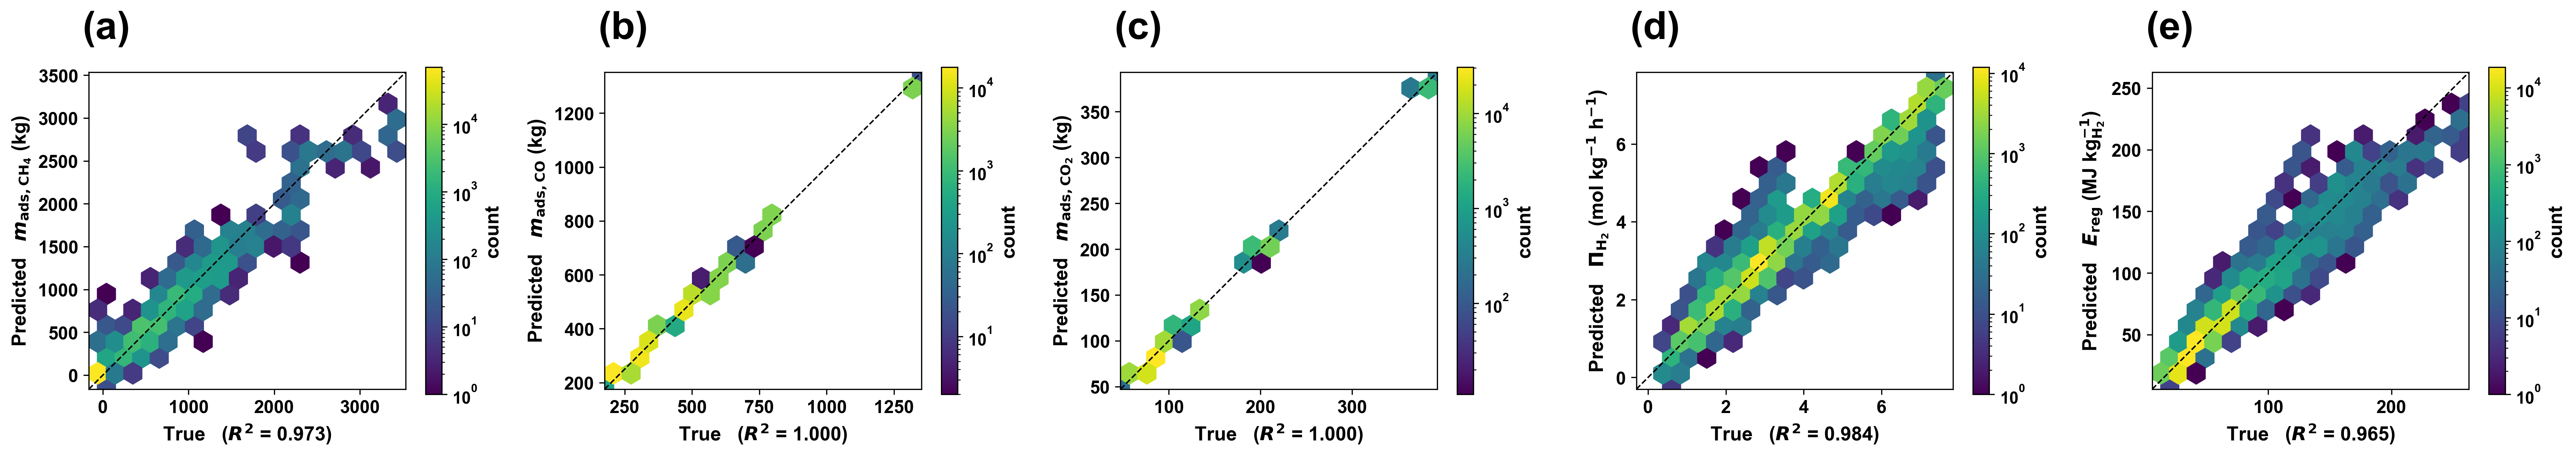
\includegraphics[width=0.98\textwidth]{../outputs/figures/si/figS_xgb_parity_random.png}
\caption{Random-row split parity plots for the XGBoost surrogate. Each panel
compares the directly computed \TSA{} scoring output with the corresponding
tree-ensemble prediction for held-out rows. Vertical banding reflects
discrete \TSA{} thermal set-points in the training data.}
\label{figS:xgbparity_random}
\end{figure}

\begin{figure}[htbp]
\centering
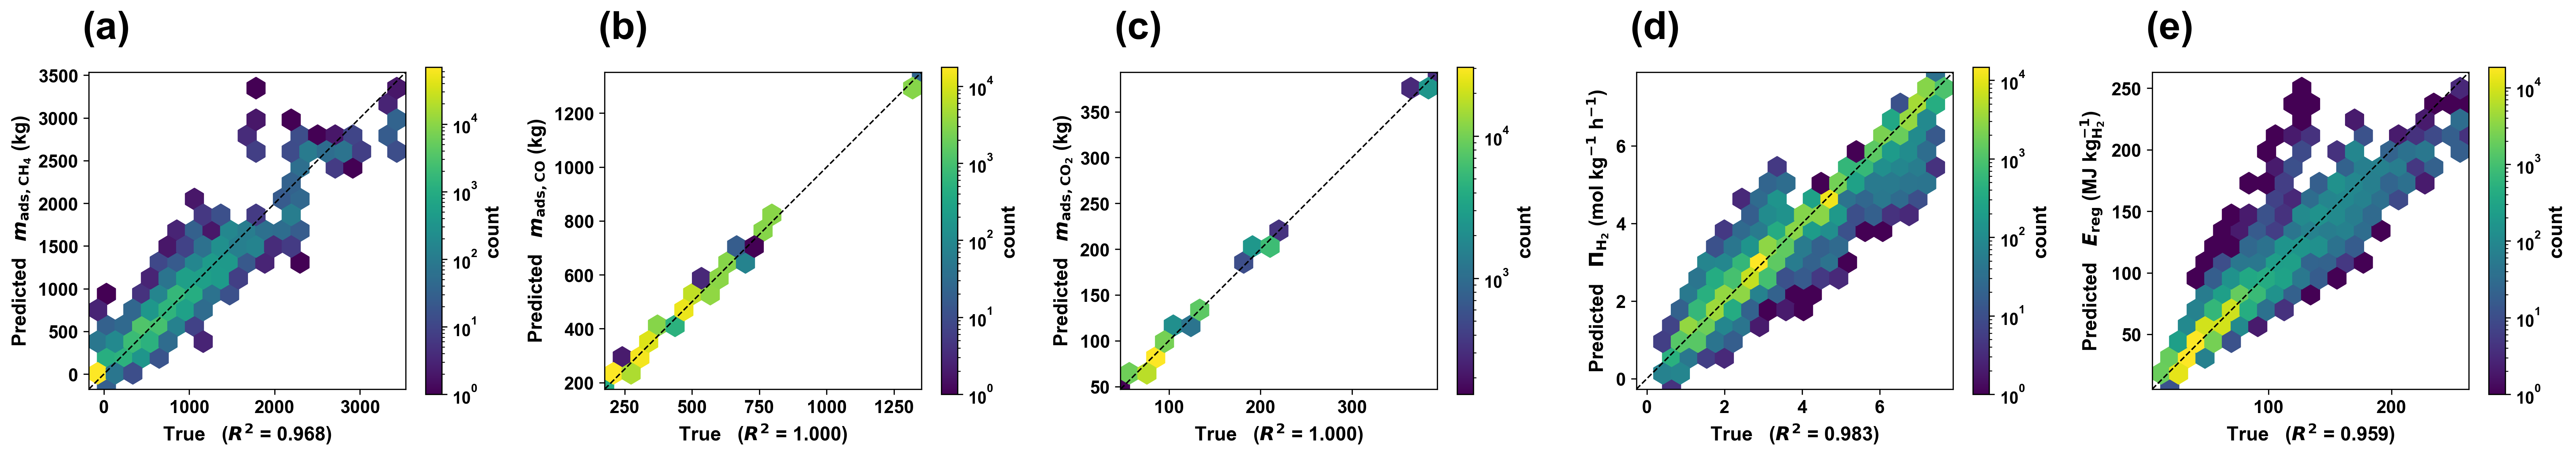
\includegraphics[width=0.98\textwidth]{../outputs/figures/si/figS_xgb_parity_grouped.png}
\caption{Gasifier-scenario-grouped split parity plots for the XGBoost
surrogate. Each panel compares the directly computed \TSA{} scoring output
with the corresponding tree-ensemble prediction for held-out gasifier
scenarios.}
\label{figS:xgbparity_grouped}
\end{figure}

\subsection{TreeSHAP attribution}

Exact TreeSHAP values were computed using XGBoost's native
\texttt{pred\_contribs} interface, which returns exact per-feature
contributions to each prediction. Mean absolute contributions across a
3{,}000-row test subsample under the grouped-split protocol are reported
in \Cref{tabS:shapvalues} and visualised in Figure~6 of the main manuscript.
Corresponding random-split attributions differ by less than one unit in
every entry, consistent with the similar held-out performance of
the two protocols.

\begin{table}[htbp]
\centering
\caption{Mean absolute TreeSHAP contribution of each controllable input to
each screening output under the gasifier-scenario-grouped split. Values are
in the units of the corresponding target. From
\texttt{shap\_mean\_abs\_all.csv}.}
\label{tabS:shapvalues}
\scriptsize
\begin{adjustbox}{max width=\textwidth}
\begin{tabular}{lccccc}
\toprule
Feature & $m_{\mathrm{ads},\CHfour}$ & $m_{\mathrm{ads},\mathrm{CO}}$ & $m_{\mathrm{ads},\COtwo}$ & $\Pi_{\Htwo}$ & $E_{\mathrm{reg}}$ \\
\midrule
Steam mass flow          & 137.1 & 4.79  & 0.681 & 0.439 & 6.41  \\
Gasifier temperature     & 192.9 & 0.162 & 0.017 & 0.455 & 7.90  \\
\TSA{} thermal set-point & 47.6  & 104.7 & 41.5  & 0.644 & 13.91 \\
Adsorbent = HKUST-1      & 2.9   & 117.6 & 2.05  & 0.734 & 2.13  \\
Adsorbent = Cu-TDPAT     & 11.7  & 17.2  & 2.35  & 0.199 & 0.583 \\
Adsorbent = Zeolite~13X  & 40.4  & 27.5  & 6.78  & 0.286 & 2.70  \\
\bottomrule
\end{tabular}
\end{adjustbox}
\end{table}

The attribution decomposes each screening output into contributions from
four process/material levers, and the dominant lever changes with the
output. \CHfour-driven inventory is dominated by upstream gasifier
set-points (steam mass flow and gasifier temperature), consistent with
methane content being set by gasification chemistry rather than adsorbent
selectivity. CO-driven inventory is dominated by adsorbent identity and by
the \TSA{} thermal set-point, consistent with CO being a regime-switching
impurity whose management depends on both material chemistry and
regeneration window. \COtwo-driven inventory is dominated by the \TSA{}
thermal set-point, matching the interpretation that \COtwo{} is a primary driver of
regeneration duty. Hydrogen productivity is distributed across all four
levers with no single dominant variable, and regeneration energy is
dominated by the \TSA{} thermal set-point with upstream contributions from
steam mass flow and gasifier temperature. This distributed structure is
the process-level basis for the regime-dependent adsorbent ranking
observed in Figure~2 of the main manuscript.

\FloatBarrier
\section{Manuscript figure-panel guide}

\Cref{tabS:panelguide} summarises the main message of the key figure panels
in the main manuscript.

\begin{table}[htbp]
\centering
\caption{Guide to the main-text figures.}
\label{tabS:panelguide}
\scriptsize
\begin{adjustbox}{max width=\textwidth}
\begin{tabular}{p{0.16\textwidth}p{0.28\textwidth}p{0.48\textwidth}}
\toprule
Figure/panel & What is plotted & Main interpretation \\
\midrule
Fig.~1 &
Process flowsheet &
Upstream gasifier and recycle choices create the \TSA{} feed; material
selection is process-coupled. \\

Fig.~2a,b &
Winner map by productivity and productivity per regeneration energy &
The gasifier operating space partitions into two ranking regimes:
Cu-TDPAT wins in \num{\approx 23}\% of scenarios and Zeolite~13X wins
in \num{\approx 77}\%; the partition is essentially unchanged when
regeneration energy is included in the ranking metric. \\

Fig.~3a--d &
\Htwo{}, \COtwo{}, \CHfour{} and CO composition maps &
Steam feed and gasifier temperature reshape the impurity hierarchy
delivered to the bed; CO-rich, \COtwo-rich and methane-influenced
regimes are distinct. \\

Fig.~4a,b &
Cu-TDPAT energy--productivity envelopes &
Cu-TDPAT approaches the high-productivity envelope under methane-limited
and thermally flexible operation, but becomes more constrained when CO
or \COtwo{} increases the retained impurity burden. \\

Fig.~4c,d &
HKUST-1 energy--productivity envelopes &
HKUST-1 occupies a lower-throughput, lower-energy region and is better
interpreted as a polishing or low-duty candidate than as a
bulk-productivity winner. \\

Fig.~4e,f &
Zeolite~13X energy--productivity envelopes &
Zeolite~13X gives the most robust global energy--productivity envelope,
especially under CO-limited operation. \\

Fig.~5a &
\CHfour-limited empirical cumulative productivity distribution &
Zeolite~13X accumulates at lower productivity, while HKUST-1 and
especially Cu-TDPAT extend into higher-productivity bands; the upper tail
of the methane-influenced productivity range is MOF-dominated. \\

Fig.~5b &
CO-limited empirical cumulative productivity distribution &
The adsorbents occupy near-non-overlapping productivity ranges, giving
the unambiguous ranking Zeolite~13X $>$ Cu-TDPAT $>$ HKUST-1 under
CO-limited operation. \\

Fig.~6 &
Mean absolute TreeSHAP attribution for the five screening outputs &
Different screening outputs are controlled by different process/material
levers; this distributed control structure explains why the binding
criterion, and therefore the winning adsorbent, changes with gasifier
regime. \\

Fig.~7a--c &
Inventory-scaled productivity for each adsorbent &
Productivity decline with adsorbent inventory introduces a secondary
footprint/inventory criterion for MOF--zeolite comparison. \\

Fig.~S14a--e &
Composite isotherms and working capacities &
\COtwo{} dominates uptake and regeneration-energy burden, while CO and
\CHfour{} act mainly as regime-switching impurities. \\
\bottomrule
\end{tabular}
\end{adjustbox}
\end{table}

\FloatBarrier
\section{Process-conditioned material-selection matrix}

\Cref{tabS:rules} translates the manuscript discussion into practical
process-conditioned material-selection rules. The rules are not intended
as design-grade column recommendations; they summarise the ranking
behaviour within the screening atlas.

\begin{table}[htbp]
\centering
\caption{Practical material-selection rules inferred from the integrated
process--adsorbent analysis.}
\label{tabS:rules}
\small
\begin{adjustbox}{max width=\textwidth}
\begin{tabular}{p{0.22\textwidth}p{0.26\textwidth}p{0.40\textwidth}}
\toprule
Operating/design regime & Preferred material & Rationale \\
\midrule
Broadly variable or CO-limited syngas &
Zeolite~13X &
Most robust high-productivity envelope; covers \num{\approx 77}\% of the
operating envelope in the winner map and gives the clearest separation
from the MOFs under CO-limited operation. \\

Methane-influenced feed with thermal-set-point leverage &
Cu-TDPAT or related tunable MOF &
Cu-TDPAT extends into the highest-productivity tail under \CHfour-limited
operation; this is the regime where MOF chemistry opens productivity
bands that are not accessed by Zeolite~13X. \\

Low-energy polishing or clean-feed operation &
HKUST-1-like MOF with moisture/CO protection &
HKUST-1 does not appear as a productivity winner in the atlas, but its
lower-throughput, lower-energy behaviour makes it relevant as a possible
polishing or low-duty candidate rather than as a bulk-productivity
material. \\

Inventory/footprint-constrained design &
Compare Cu-TDPAT and Zeolite~13X by productivity decay with
$m_{\mathrm{ads,max}}$ &
Maximum productivity alone favours Zeolite~13X in most regimes, but
inventory-scaled productivity can make a MOF more attractive when bed
mass, footprint or thermal-management constraints become important. \\

Future hybrid-bed design &
Zeolite guard layer plus MOF polishing/high-capacity layer &
Combines zeolite robustness with MOF tunability; the crossover boundary
identified in the winner map is the most useful region for testing
whether a layered or hybrid bed can outperform either adsorbent alone. \\
\bottomrule
\end{tabular}
\end{adjustbox}
\end{table}

\FloatBarrier
\section{Pressure-swing robustness check}
\label{secS:vsa}

To test whether the ranking crossover reported in the main manuscript is
specific to a thermal-swing regeneration mechanism, the same equilibrium
working-capacity scoring model was applied to a vacuum-swing variant. In
this variant, the adsorption phase is fixed at \SI{1}{bar} and the
desorption endpoint is swept over \SIrange{0.01}{0.63}{bar}. Ten
desorption-pressure states were exported, paired one-to-one with ten
temperature states in the export macro; because the pressure-swing scoring
formulas do not depend on those temperature cells, the resulting table is
a clean desorption-pressure sweep.

The scoring model is otherwise identical to Eqs.~\eqref{eqS:langmuir}--\eqref{eqS:prod}
of this Supporting Information. The pressure-swing table is used only to test
whether the adsorbent-ranking partition is preserved when the swing variable is
changed from temperature to pressure. It is not a complete PSA/VSA process
model: compressor work, vacuum-pump work, pressure-drop losses and detailed
cycle scheduling are not included. Absolute pressure-swing energy values are
therefore not compared with \TSA{} energy values in the manuscript.

\Cref{figS:vsa_winner} shows the resulting winner map. Cu-TDPAT occupies
\num{22.86}\% of gasifier scenarios and Zeolite~13X occupies
\num{77.14}\%, essentially identical to the \TSA{} shares of
\num{22.90}\% and \num{77.10}\% reported in the main manuscript. HKUST-1
does not appear as a productivity winner under either scoring, consistent
with its role as a lower-throughput, lower-energy candidate. The
qualitative similarity of the two partitions supports the narrower conclusion
that the crossover is not tied to the thermal swing variable alone. Within the
equilibrium scoring framework, it is mainly associated with the gasifier-derived
impurity hierarchy and the relative material working capacities.

\begin{figure}[htbp]
\centering
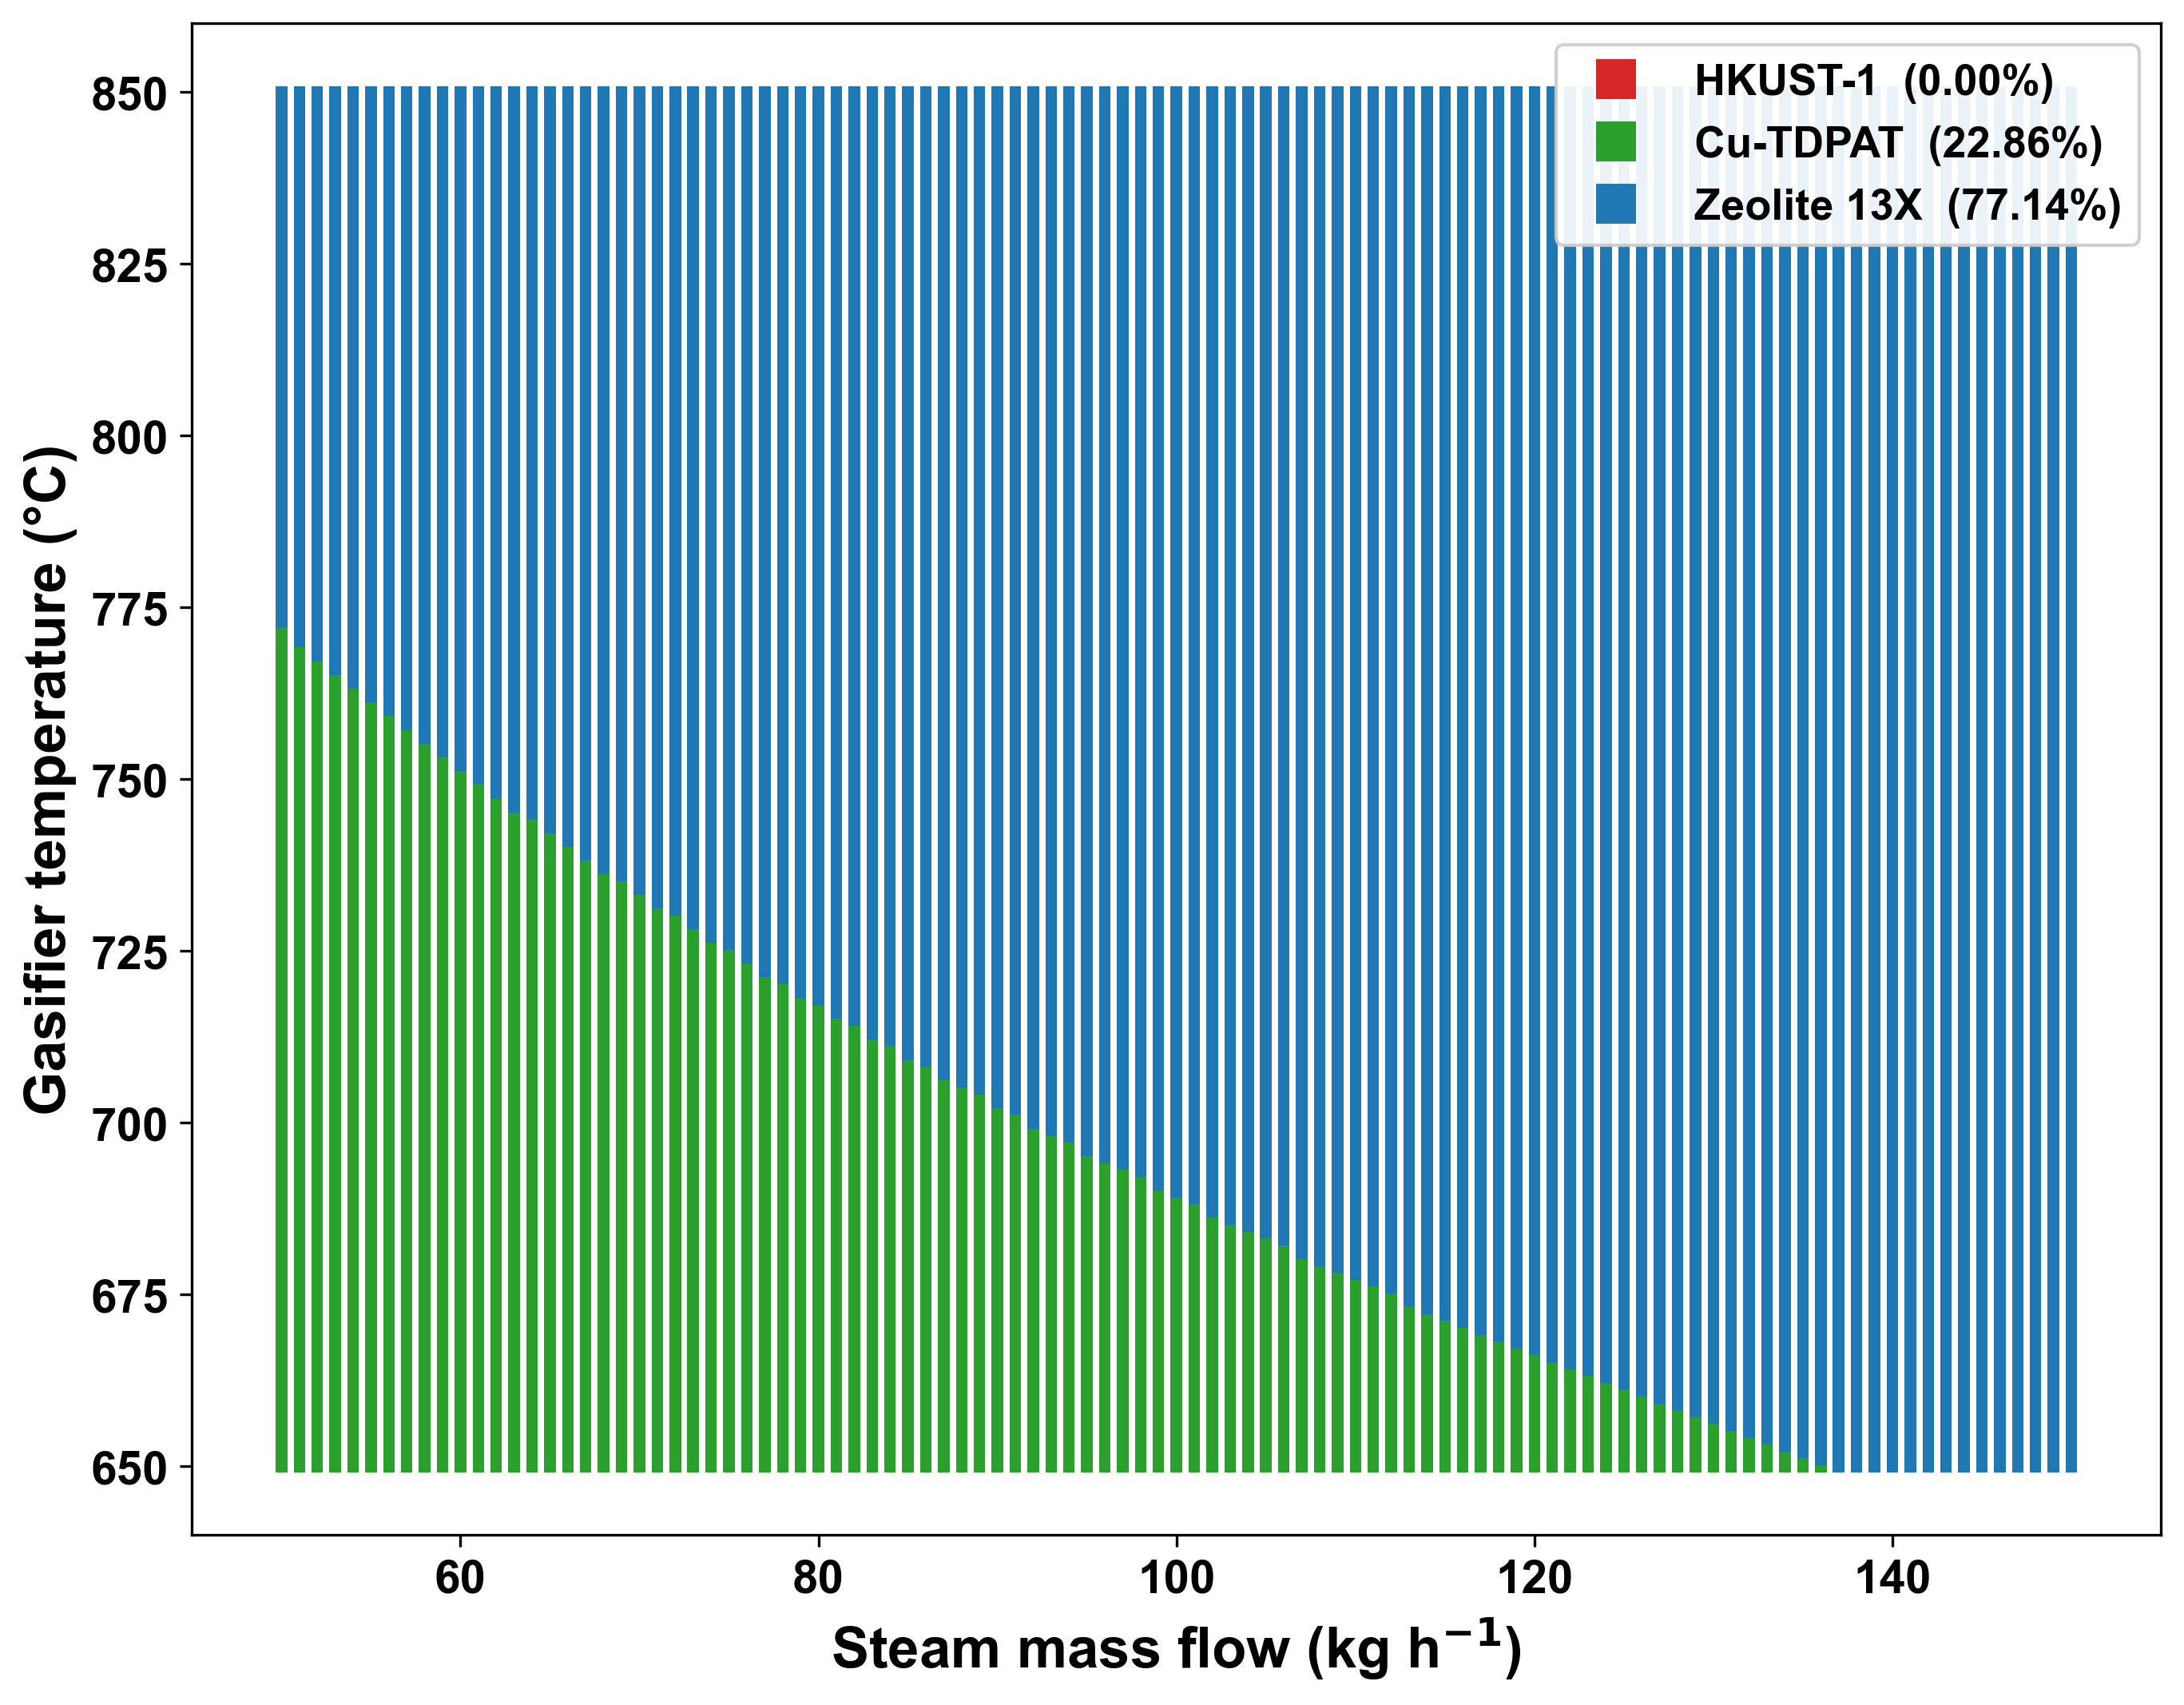
\includegraphics[width=0.90\textwidth]{../outputs/figures/si/figS_vsa_winner_map.png}
\caption{Vacuum-swing robustness check. Adsorbent winner map on the
gasifier operating plane under the pressure-swing scoring variant
(adsorption at \SI{1}{bar}, desorption endpoint swept over
\SIrange{0.01}{0.63}{bar}). Cu-TDPAT wins \num{22.86}\% of scenarios,
Zeolite~13X wins \num{77.14}\%, and HKUST-1 does not appear as a winner
under either scoring. The partition is essentially identical to the
\TSA{} winner map (Fig.~2 of the main manuscript), consistent with the
interpretation that the ranking crossover is controlled by the impurity
hierarchy and relative material working capacities rather than by the
specific swing variable in the equilibrium scoring rule.}
\label{figS:vsa_winner}
\end{figure}

\FloatBarrier
\section{Robustness of the ranking partition to $\eta$ and $t_{\mathrm{cycle}}$ choices}
\label{secS:robustness}

Two model parameters could plausibly be argued as arbitrary: the imposed
impurity-removal factor $\eta_i$ and the cycle time $t_{\mathrm{cycle}}$.
The manuscript uses $\eta_i = 0.99$ (uniform) and $t_{\mathrm{cycle}} =
\SI{900}{s}$ throughout. \Cref{tabS:robustness} reports the winner-map
shares under three classes of perturbation.

Under uniform $\eta$ scaling (0.90, 0.95, 0.99, 0.999) and uniform
$t_{\mathrm{cycle}}$ scaling (600 s, 900 s, 1500 s), the shares are
identically 22.86\% (Cu-TDPAT) and 77.14\% (Zeolite~13X) in every case,
matching the baseline. Under non-uniform $\eta$ (industrially motivated
combinations: 99.99\% CO removal / 99\% CO$_2$ removal / 95\% CH$_4$
removal; two other stringency combinations), the shares are again exactly
22.86\%/77.14\%. \Cref{figS:robustness_eta} confirms visually that the
winner map is identical across baseline and non-uniform $\eta$ cases.

This exact invariance is a direct consequence of the scoring structure.
From Eqs.~\eqref{eqS:arrhenius}--\eqref{eqS:mads}, the impurity-specific
mass requirement is $m_{\mathrm{ads},i} = n_{i,\mathrm{feed}}\eta_i /
\Delta q_i$ and the controlling inventory is $m_{\mathrm{ads,max}} =
\max_i(m_{\mathrm{ads},i})$. When $\eta_i$ scales by a factor common to
all adsorbents (uniform or non-uniform in $i$ but the same for HKUST-1,
Cu-TDPAT and Zeolite~13X), $m_{\mathrm{ads},i}$ for each adsorbent scales
by the same factor and the ratio between adsorbents at a given scenario
is preserved. The adsorbent with the highest productivity per unit
adsorbent mass therefore remains the same. Similarly, $t_{\mathrm{cycle}}$
enters the productivity denominator uniformly for all adsorbents and does
not change the winner.

The winner-map partition is therefore not sensitive to the specific
$\eta_i$ or $t_{\mathrm{cycle}}$ values chosen. This result should be
interpreted narrowly: it shows that the partition is not an artefact of the
selected removal target or cycle-time choice. It does not, by itself, validate
the gasification reactor-conversion assumptions; those assumptions determine
the feed-composition family to which the adsorbent score is then applied.

\begin{table}[htbp]
\centering
\caption{Sensitivity of the winner-map partition to $\eta$ and
$t_{\mathrm{cycle}}$ perturbations. All eight tested conditions give
identical winner shares to the baseline. This exact invariance follows
analytically from the scoring structure of
Eqs.~\eqref{eqS:arrhenius}--\eqref{eqS:mads} (see discussion in
Section~\ref{secS:robustness}). The result demonstrates invariance to the
removal-target and cycle-time normalisations tested here; it should not be
read as independent validation of the upstream gasification-conversion
assumptions.}
\label{tabS:robustness}
\small
\begin{adjustbox}{max width=\textwidth}
\begin{tabular}{llccc}
\toprule
Sensitivity & Condition & HKUST-1 (\%) & Cu-TDPAT (\%) & Zeolite~13X (\%) \\
\midrule
Baseline           & $\eta_i = 0.99$, $t_{\mathrm{cycle}} = \SI{900}{s}$ & 0.00 & 22.86 & 77.14 \\
Uniform $\eta$     & $\eta_i = 0.900$          & 0.00 & 22.86 & 77.14 \\
Uniform $\eta$     & $\eta_i = 0.950$          & 0.00 & 22.86 & 77.14 \\
Uniform $\eta$     & $\eta_i = 0.999$          & 0.00 & 22.86 & 77.14 \\
Non-uniform $\eta$ & strict CO (0.9999)        & 0.00 & 22.86 & 77.14 \\
Non-uniform $\eta$ & strict CO + CO$_2$        & 0.00 & 22.86 & 77.14 \\
Non-uniform $\eta$ & strict CO$_2$ only        & 0.00 & 22.86 & 77.14 \\
Cycle time         & $t_{\mathrm{cycle}} = \SI{600}{s}$ & 0.00 & 22.86 & 77.14 \\
Cycle time         & $t_{\mathrm{cycle}} = \SI{1500}{s}$ & 0.00 & 22.86 & 77.14 \\
\bottomrule
\end{tabular}
\end{adjustbox}
\end{table}

\begin{figure}[htbp]
\centering
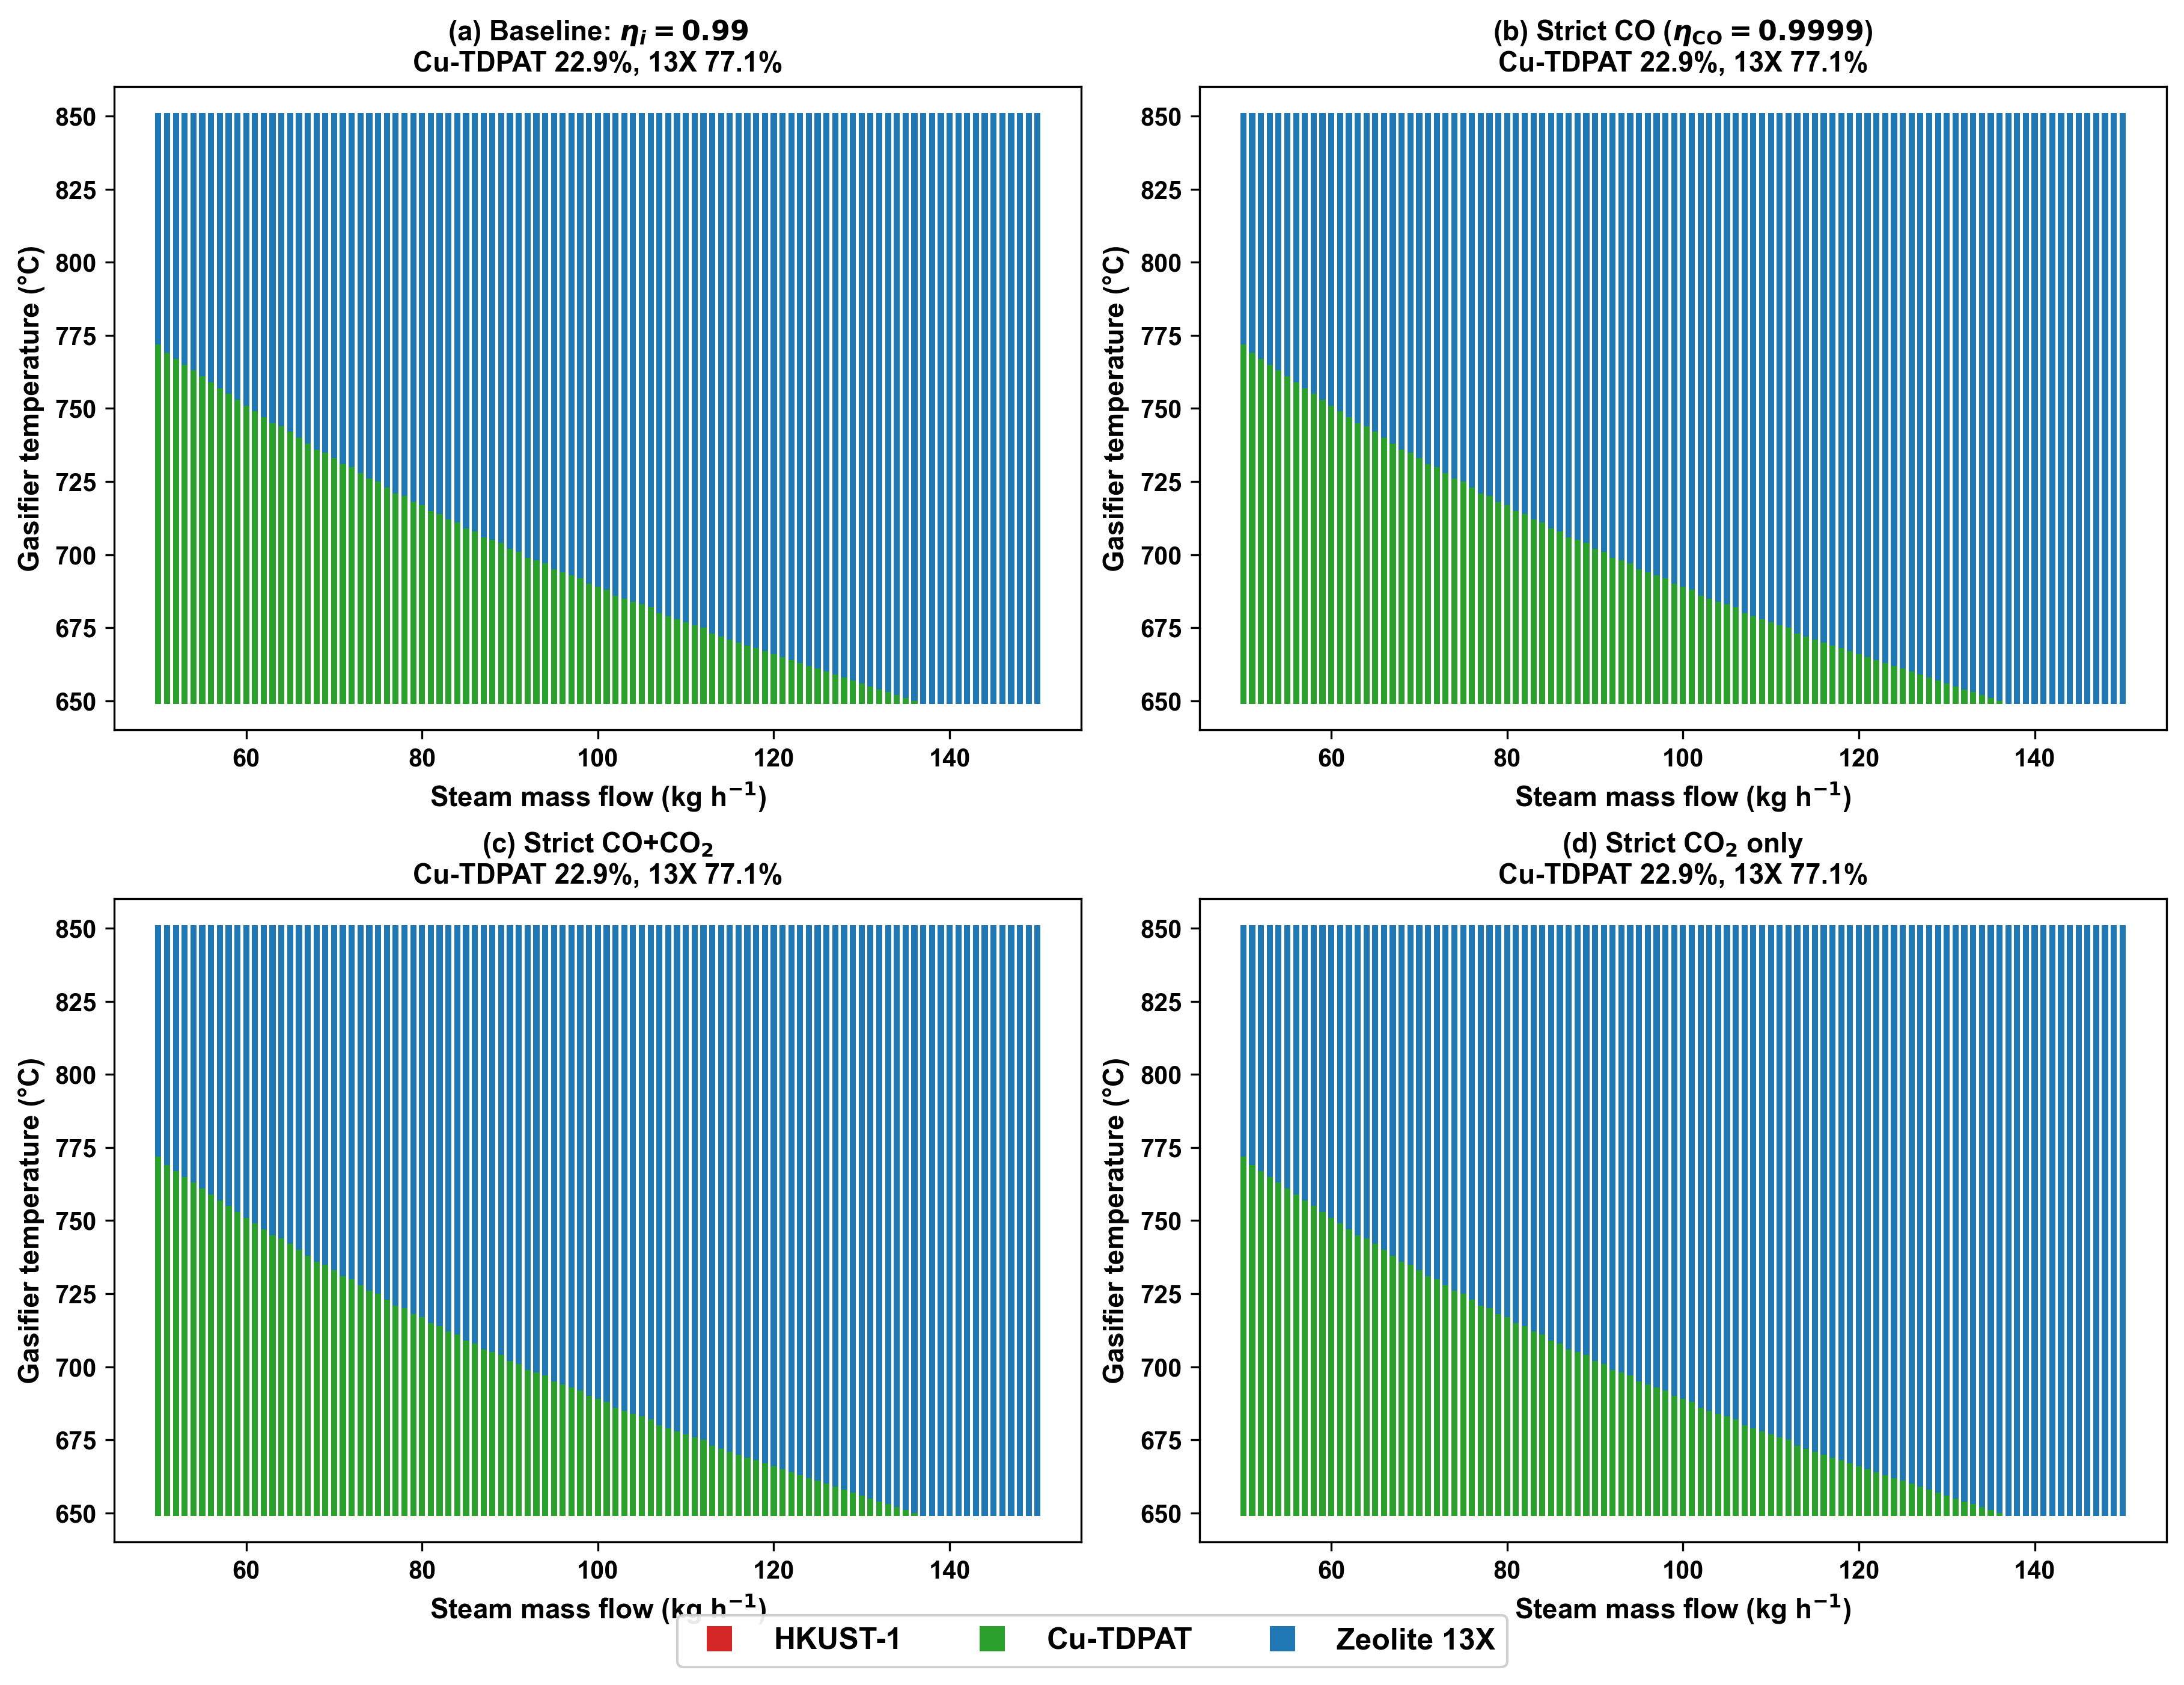
\includegraphics[width=0.95\textwidth]{../outputs/figures/si/figS_robustness_eta_sensitivity.png}
\caption{Winner maps under (a) baseline $\eta_i = 0.99$, (b) strict CO
removal ($\eta_{\mathrm{CO}} = 0.9999$, $\eta_{\CHfour} = 0.95$),
(c) strict CO+CO$_2$ ($\eta_{\mathrm{CO}} = \eta_{\COtwo} = 0.9999$),
and (d) strict CO$_2$ only ($\eta_{\COtwo} = 0.9999$). All four panels
give identical winner-share partitions (Cu-TDPAT 22.86\%, Zeolite~13X
77.14\%). The visual identity of the four maps demonstrates that the
regime-conditional adsorbent-ranking finding is not sensitive to the
industrial removal-target profile.}
\label{figS:robustness_eta}
\end{figure}


\newpage

\begin{figure}[htbp]
  \centering
  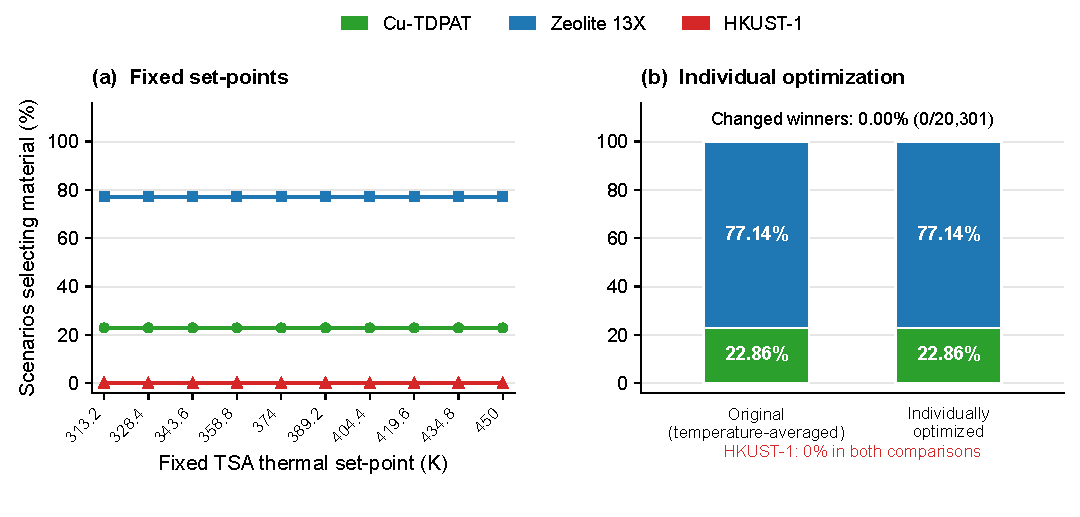
\includegraphics[width=\textwidth]{../outputs/figures/si/tsa_temperature/figS19_r1c5.pdf}
  \caption{\add{Effect of TSA thermal set-point selection on productivity-based material winners across 20,301 gasifier scenarios. (a) Percentages selecting Cu-TDPAT, Zeolite 13X and HKUST-1 at each of the ten fixed thermal set-points (313.2, 328.4, 343.6, 358.8, 374.0, 389.2, 404.4, 419.6, 434.8 and 450.0~K). Every fixed set-point gives 22.8560\%, 77.1440\% and 0\%, respectively, with no scenario winner changed from the original map. (b) Original temperature-averaged winner proportions versus those obtained by maximizing productivity over the ten saved set-points independently for each material and scenario before selecting the material. Individual optimization changes 0 of 20,301 winners (0\%). The original map is a screening comparison, not an operating strategy. All comparisons use the existing TSA results.}}
  \label{fig:tsa-temperature-winners}
\end{figure}

\bibliographystyle{unsrtnat}
\bibliography{references}

\end{document}